\documentclass[letterpaper,11pt]{report}
\usepackage[pdftex]{graphicx}
\usepackage{epstopdf}
%\usepackage[dvips]{graphicx}
\usepackage{epsfig,float,captdef,multicol,amssymb,amsmath,amsfonts}
\usepackage[activeacute,spanish]{babel}

%\usepackage[latin1]{inputenc}
\usepackage[colorlinks]{hyperref}

\usepackage{cancel}
\usepackage{marginnote}
\renewcommand*{\marginnotevadjust}{-0.1cm}
\renewcommand*{\marginfont}{\footnotesize}
%\renewcommand*{\marginfont}{\tiny}
\usepackage[right=4.5cm,left=2cm,top=2cm,bottom=2.0cm,headsep=0.7cm,footskip=1.0cm]{geometry}

%\usepackage[notref]{showkeys} % muestra los labels de las referencias.

\def\refname{Referencias}
\def\abstractname{Resumen}
\def\bibname{Referencias}
\def\chaptername{Cap{\'\i}tulo}
\def\appendixname{Ap'endice}
\def\contentsname{\'Indice}
\def\listfigurename{\'Indice de Figuras}
\def\listtablename{\'Indice de Tablas}
\def\indexname{\'Indice de Materias}
\def\figurename{Figura}
\def\tablename{Tabla}
\def\partname{Parte}
\def\enclname{Adjunto}
\def\ccname{Copia a}
\def\headtoname{A}
\def\headpagename{P\'agina}
\def\today{\number\day~de\space\ifcase\month\or
 enero\or febrero\or marzo\or abril\or mayo\or junio\or
 julio\or agosto\or septiembre\or octubre\or noviembre\or diciembre\fi
 \space de~\number\year}


%\topmargin -0.5cm  %regula margen superior (desde donde comienza a escribir)
%\headheight 10pt
%\headsep 0.6cm
%\textheight 22.5cm %regula el alto del texto



\begin{document}

\thispagestyle{empty}
\begin{center}

\

\vspace{6.5cm}

\rule{15cm}{0.1cm}

\vspace{1.5cm}

{\huge \textsc{\textbf{Grupos y Simetr\'ias}}}

\vspace{1.5cm}

\rule{15cm}{0.1cm}
\vspace{1.5cm}

Versi'on del \today

\end{center}


\newpage
\thispagestyle{empty}
\ \\
\newpage


\tableofcontents
\pagenumbering{arabic}
\setcounter{page}{1}
\chapter{Simetr'ias y Teor'ia de Grupos}
\section{Elementos de Teor'ia de Grupos}

Decimos que una colecci'on de elementos $g_i\in G$ forman un \textit{grupo} si ellos satisfacen las siguientes propiedades:
\begin{enumerate}
\item Clausura bajo una operaci'on de composici'on: Si $g_i,g_j\in G$, entonces $g_i\cdot g_j\in G$.
\item Asociatividad bajo la composici'on: $\forall g_i,g_j,g_k\in G$, 
$g_i\cdot (g_j\cdot g_k)=(g_i\cdot g_j)\cdot g_k$.

\item Existencia de Elemento \textit{identidad}: existe un elemento $\mathbb{I}$ tal que $\forall g_i\in G$ satisface $g_i\cdot \mathbb{I}=\mathbb{I}\cdot g_i=g_i$.
\item Existencia de Elemento \textit{inverso}: $\forall g_i\in G$ existe un elemento $g_i^{-1}\in G$ tal que $g_i \cdot g_i^{-1}=g_i^{-1} \cdot g_i=\mathbb{I}$.
\end{enumerate} 

Existen varios tipos de grupos. Un \textit{grupo discreto} tiene un n'umero finito de elementos. Sin embargo, estamos m'as interesados en los grupos continuos, como el grupo de rotaci'on y el grupo de Lorentz, los cuales dependen de un conjunto de par'ametros continuos.

\subsection{Grupos de Lie}

\subsection{$SO(2)$}

El grupo $O(2)$ o rotaciones en dos dimensiones.
Si rotamos el plano en un 'angulo $\theta$, luego las coordenadas $(x^\prime,y^\prime)$ del mismo punto en el nuevo sistema coordenado son dadas por:
\begin{equation}
\begin{pmatrix}x^{\prime}\\
y^{\prime}
\end{pmatrix}=\begin{pmatrix}\cos\theta & \sen\theta\\
-\sen\theta & \cos\theta
\end{pmatrix}\begin{pmatrix}x\\
y
\end{pmatrix}.
\end{equation}
Podemos abreviar esto como:
\begin{equation}
x^{i\prime}=O^{ij}(\theta)x^j.
\end{equation}
Para 'angulos peque\~nos, podemos reducir esto a
\begin{equation}
\delta x=\theta y;\,\,\,\, \delta y=-\theta x
\end{equation}
o simplemente
\begin{equation}
\delta x^i=\theta \epsilon^{ij}x^j,
\end{equation}
donde $\epsilon^{ij}$ es antisim'etrica. Estas matrices forman un grupo; por ejemplo, podemos escribir la inversa de alguna rotaci'on, dada por $O^{-1}(\theta)=O(-\theta):$
\begin{equation}
O(\theta)O(-\theta)=\mathbb{I}=\begin{pmatrix}1 & 0\\
0 & 1
\end{pmatrix}.
\end{equation}
El hecho de que estas matrices preserven invariante la longitud da lugar a restricciones sobre ellas. Para encontrar la naturaleza de estras restricciones, hagamos una rotaci'on sobre la distancia invariante:
\begin{equation}
\begin{aligned}
x^{i\prime}x^{i\prime}&=&O^{ij}x^jO^{ik}x^k \\
&=&x^j\left(O^{ij}O^{ij}\right)x^k \\
&=& x^jx^j,
\end{aligned}
\end{equation}
entonces esto es invariante si la matriz $O$ es ortogonal
\begin{equation}
O^{ij}O^{ij}=\delta^{jk}.
\end{equation}
Para tomar el inverso de una matriz ortogonal, simplemente tomamos la transpuesta. El grupo de rotaciones $O(2)$ es llamado grupo ortogonal en dos dimensiones, de hecho, puede ser definido como un conjunto de matrices reales dos dimensional matrices ortogonales. Cualquier matriz ortogonal puede ser escrita como la exponenciaci'on de un matriz antisim'etrica $\tau$
\begin{equation}
O(\theta)=e^{\theta\tau}=\sum_{n=0}^\infty \frac{1}{n!}(\theta\tau)^n,
\end{equation}
donde
\begin{equation}
\tau=\begin{pmatrix}0 & 1\\
-1 & 0
\end{pmatrix}.
\end{equation}
Todos los elementos de $O(2)$ son parametrizados por un 'unico 'angulo $\theta$. Decimos que $O(2)$ es un grupo uniparam'etrico, esto es, tiene dimensi'on 1. 
Consideremos ahora el determinante a ambos lados de la ecuaci'on, es decir
\begin{equation}
\det (OO^T)=\det O \det O^T =(\det O)^2=1.
\end{equation}
Esto significa que el determinando de $O$ es igual a $\pm 1$. Si tomamos $\det O=1$, el subgrupo resultante es llamado $SO(2)$. Las rotaciones que hemos visto entonces son miembros de $SO(2)$. Sin embargo, si tomamos ahora $\det O=-1$ esto no forman un grupo, puesto que no posee al elemento identidad.


\section{Representaciones}
Si $g_i$ es un miembro de un grupo $G$, entonces el objeto $D(g_i)$ es llamado representaci'on de $G$ si obedece:
\begin{equation}
D(g_i)D(g_j)=D(g_ig_j)
\end{equation}
para todos los elementos en el grupo. En otras palabras, $D(g_i)$ tiene las mismas reglas de multiplicaci'on  que el grupo original.
Una representaci'on es llamada reducible si $D(g_i)$ se puede poner en forma diagonal. Por ejemplo, la siguiente matriz es una representaci'on reducible
\begin{equation}
D(g_{i})=\begin{pmatrix}D_{1}(g_{i}) & 0 & 0\\
0 & D_{2}(g_{i}) & 0\\
0 & 0 & D_{3}(g_{i})
\end{pmatrix}
\end{equation}
donde $D_i$ son representaciones m'as peque\~nas del grupo.
El principal objetivo es encontrar las representaciones irreducibles de los grupos en cuesti'on. 
%Esto es porque los campos b'asicos de la f'isica transforman como representaciones irreducibles de los grupos de Lorentz y Poincar'e. 
En particular, una manera de generar representaciones mayores de $O(2)$ es simplemente multiplicar vectores. El producto $A^iB^j$, por ejemplo, transforma como
\begin{equation}
A^{i\prime}B^{j\prime}=\left[O^{i\prime i}(\theta)O^{j\prime j}(\theta)\right]A^iB^j.
\end{equation}
Esta matriz $O^{i\prime i}(\theta)O^{j\prime j}(\theta)$ forma una representaci'on de  $SO(2)$. Tiene la misma regla de multiplicaci'on que $O(2)$, pero el espacio sobre el que act'ua es $2\times 2$ dimensional.
En general, un tensor $T^{ijk\cdots}$ bajo $O(2)$ no es nada en particular pero un objeto que transforma como el producto de una serie de vectores ordinarios.
La transformacion de $T^{ijk\cdots}$ es id'estica a la transformaci'on del producto $x^ix^jx^k\cdots.$ Este producto forma una representaci'on de $O(2)$ dado que
\begin{equation}
O^{i_1,i_2\cdots i_N;j_1,j_2\cdots j_N}(\theta)=O^{i_1,j_1}(\theta)O^{i_2,j_2}(\theta)\cdots O^{i_N,j_N}(\theta)
\end{equation}
tiene la misma regla de multipilaci'on que $SO(2)$.
Un conveniente m'etodo que se usa para crear representaciones irreducibles es usar dos tensores bajo $O(2)$ que son constantes: $\delta^{ij}$ y $\epsilon^{ij}$, donde $\epsilon^{12}=-\epsilon^{21}=1$.
Podemos mostrar la equivalencia entre $O(2)$ y otra formulaci'on. Tomemos un objeto complejo $u=a+ib$, que transforma de la siguiente manera:
\begin{equation}
u^\prime = U(\theta)u=e^{i\theta}u.
\end{equation}
La matriz $U(\theta)$ es llamada matriz unitaria, porque
\begin{equation}
U\times U^\dagger = \mathbb{I}.
\end{equation}
El conjunto de todas las matrices unitarias unidimensionales $U(\theta)=e^{i\theta}$ definen un grupo llamado $U(1)$. Si hacemos dos transformaciones encontramos
\begin{equation}
e^{i\theta}e^{i\theta^\prime}=e^{i\theta+i\theta^\prime},
\end{equation}
donde tenemos la misma ley de multiplicaci'on que $O(2)$, aunque esta construcci'on es basada en un nuevo espacio, el espacio de n'umeros complejos unidimensionales. Luego decimos que
\begin{equation}
SO(2)\sim U(1).
\end{equation}
Esto significa que hay una correspondencia entre las dos, aunque ellas est´an definidas en dos diferentes espacios
\begin{equation}
e^{\tau(\theta)}\leftrightarrow e^{i\theta}.
\end{equation}
Para ver la correspondencia entre $O(2)$ y $U(1)$, consideremos dos campos escalares $\phi_1$ y $\phi_2$ que transforman infinitesimalmente bajo $SO(2)$, es decir
\begin{equation}
\delta\phi_i = \theta \epsilon^{ij}\phi_j
\end{equation}
lo cual es justamente la regla de transformaci'on para $\theta$ peque\~no. Dado $SO(2) \sim U(1),$ los campos escalares pueden ser combinados dentro de un campo escalar complejo
\begin{equation}
\phi =\frac{1}{\sqrt{2}}\left(\phi_1+i\phi_2\right).
\end{equation}
Luego la variaci'on infinitesimal de este campo bajo $U(1)$ es dado por
\begin{equation}
\delta \phi =-i\theta \phi
\end{equation}
para $\theta$ peque\~no.


\subsection{Representaciones de $SO(3)$ y $SU(2)$} 
El grupo $O(2)$ fue f'acil de analizar puesto que sus elementos conmutan entre ellos. A estos grupos los llamamos grupos Abelianos. Ahora repasaremos grupos no-Abelianos, donde los elementos no necesariamente conmutan entre ellos. Definimos $O(3)$ como el grupo que deja la distancia invariante en tres dimensiones, es decir
\begin{equation}
\quad \text{Invariante:}\,\,\,\,\,  x^2+y^2+z^2
\end{equation}
donde $x^{i\prime}=O^{ij}x^j$. Si repetimos los pasos que hicimos para $SO(2)$, sabemos que el conjunto de matrices $3\times 3$, reales y ortogonales $O(3)$ deja invariante esta cantidad. La condici'on de ortogonalidad reduce el n'umero de n'umeros independientes a $9-3=6$. Cualquier miembro de $O(3)$ puede ser escrito como la exponencial de una matriz antisim'etrica
\begin{equation}
O=\exp \left({i\sum_{i=1}^{3}\theta^i \tau^i}\right),
\end{equation}
donde $\tau^i$ son elementos puramente imaginarios. As'i hay tres matrices antisim'etricas $3\times 3$ independientes. Por lo tanto $O(3)$ es un grupo de Lie de tres par'ametros, parametrizados por tres ángulos.
Estas tres matrices antisim'etricas $\tau^i$ pueden ser escritas como:
\begin{equation}
\begin{aligned}
\tau^{1}=-i\begin{pmatrix}0 & 0 & 0\\
0 & 0 & 1\\
0 & -1 & 0
\end{pmatrix};\,\,\,\,\,\,\tau^{2}=-i\begin{pmatrix}0 & 0 & -1\\
0 & 0 & 0\\
1 & 0 & 0
\end{pmatrix}, \\
\tau^{3}=-i\begin{pmatrix}0 & 1 & 0\\
-1 & 0 & 0\\
0 & 0 & 0
\end{pmatrix}.
\end{aligned}
\end{equation}
Se puede probar que este conjunto de matrices puede ser representado por el tensor antisim'etrico $\epsilon^{ijk}$ como
\begin{equation}
(\tau^i)^{jk}=-i\epsilon^{ijk}
\end{equation}
donde $\epsilon^{123}=1$. Estas matrices antisim'etricas, obedecen a la siguiente propiedad:
\begin{equation}
[\tau^i,\tau^j]=i\epsilon^{ijk}\tau^k. \label{algebraso3}
\end{equation}
Este es un ejemplo de un 'algebra de Lie. Las constantes $\epsilon^{ijk}$ que aparecen en el 'algebra son llamadas constantes de estructura del 'algebra. Una determinaci'on completa de las constantes de estructura de alg'un 'algebra  especifican el 'algebra de Lie, y tambi'en el grupo que est'a por detr'as.
Para 'angulos peque\~nos $\theta^i$, podemos escribir la ley de transformaci'on como
\begin{equation}
\delta x^i=\epsilon^{ijk}\theta^k x^j.
\end{equation}
Introduciendo los operadores
\begin{equation}
L^i\equiv i\epsilon^{ijk} x^j \partial^k
\end{equation}
podemos mostrar que la relaci'on de conmutaci'on de los $L^i$ satisfacen la de $SO(3)$. Construyendo el operador
\begin{equation}
U(\theta)=e^{i\theta^i L^i},
\end{equation}
un campo escalar y vectorial, transforman como
\begin{equation}
\begin{aligned}
U(\theta^k \phi(x)U^{-1}(\theta^k)&=&\phi(x^\prime), \\
U(\theta^k \phi^i(x)U^{-1}(\theta^k)&=&\left(O^{-1}\right)^{ij}(\theta^k)\phi^j(x^\prime).
\end{aligned}
\end{equation}
Como en el caso de $O(2),$ podemos encontrar la relaci'on entre $O(3)$ y el grupo unitario. Considerando el conjunto de todas mas matrices unitarias, con determinante 1 de $2\times 2$. Estas matrices forman un grupo, llamado $SU(2)$, el cual es tambi'en llamado el grupo unitario especial en dos dimensiones. Estas matrices tienen 3 elementos independientes. Una matriz unitaria puede ser escrita como la exponencial de una matriz hert'itica $H$, donde $H=H^\dagger$,
\begin{equation}
U=e^{iH}.
\end{equation}
Para probar esta relaci'on, simplemente tomamos el herm'itico conjugado a ambos lados de la ecuaci'on, es decir
\begin{equation}
\begin{aligned}
U^{\dagger}&=&e^{-iH^{\dagger}} \\
&=&e^{-iH} \\
&=&U^{-1}.
\end{aligned}
\end{equation}
Puesto que un elemento de $SU(2)$ puede ser parametrizado por tres n'umeros, el conjunto m'as conveniente es usar las conocidas matrices de Pauli. Cualquier elemento de $SU(2)$ puede ser escrito como
\begin{equation}
U=e^{i\theta^i \sigma^i /2},
\end{equation}
donde
\begin{equation}
\sigma^{1}=\begin{pmatrix}0 & 1\\
1 & 0
\end{pmatrix};\,\,\,\sigma^{2}=\begin{pmatrix}0 & -i\\
i & 0
\end{pmatrix};\,\,\,\sigma^{3}=\begin{pmatrix}1 & 0\\
0 & -1
\end{pmatrix}
\end{equation}
donde $\sigma^i$ safisfacen la relaci'on:
\begin{equation}
\left[\frac{\sigma^i}{2},\frac{\sigma^j}{2}\right]=i\epsilon^{ijk}\frac{\sigma^k}{2}.
\end{equation}
Ahora, tenemos exactamente la misma 'algebra que para $SO(3)$ en la ecuaci'on \eqref{algebraso3}. Por lo tanto, podemos decir que
\begin{eqnarray}
SO(3) \sim SU(2).
\end{eqnarray}

%\section{El Grupo de Poincar'e}



\chapter{El Grupo de Lorentz}\label{appLor}
\section{Definici'on y generalidades}

En el contexto de la teor{'i}a Especial de la Relatividad (RE), un punto
(vector) de la variedad espacio-tiempo ({\em espacio de Minkowski}, $M_{4}$)
es caracterizado, en un sistema de referencia inercial (SRI) $O$, por las
coordenadas espacio-temporales cartesianas $x^{\mu
}=(x^0,x^1,x^2,x^3)=(t,x,y,z)=(t,x^{i})=(t,\vec{x})$.

Una Tranformaci'on de Lorentz (TL) es una transformaci'on lineal, real
y homog'enea de la forma 
\begin{equation}
x^{\mu }\rightarrow \widetilde{x}^{\mu }=\Lambda _{\nu }^{\mu }x^{\nu },
\label{tl}
\end{equation}
o en notaci'on matricial 
\begin{equation}
\widetilde{{\bf x}}={\bf \Lambda x,}
\end{equation}
tal que la forma cuadRatica 
\begin{equation}
s^2=\eta _{\mu \nu }x^{\mu }x^{\nu }=t^2-x^2-y^2-z^2,\qquad \eta
_{\mu \nu }={\rm diag}(1,-1,-1,-1),  \label{il}
\end{equation}
\newline
permanece invariante. Esto implica que las matrices ${\bf \Lambda }$ deben
satisfacer la condici'on 
\begin{equation}
\eta _{\mu \nu }\Lambda _{\lambda }^{\mu }\Lambda _{\rho }^{\nu }=\eta
_{\lambda \rho },  \label{indic}
\end{equation}
es decir, 
\begin{equation}
{\bf \Lambda }^{\top }{\bf \eta \Lambda =\eta }.  \label{condinv}
\end{equation}

F{\'{\i }}sicamente una TL de la forma (\ref{tl}) representa una
transformaci'on entre dos SRI's $O\rightarrow \widetilde{O}$ (vinculados
respectivamente a las coordenadas $x$ y $\widetilde{x}$). La condici'on
anterior expresa la equivalencia f{\'{\i }}sica de los sistemas de
referencia $O$ y $\widetilde{O}$ (ppio. de relatividad), y en particular la
existencia de una simetr{\'{\i }}a fundamental entre las tres dimensiones
espaciales y la dimensi'on temporal, las cual es manifestada en la
constancia de la velocidad (rapidez) de la luz en todos los SRI's\footnote{%
Aqu{\'{\i }} consideramos el sistema ``geometrizado'' de unidades, en el que 
$c\equiv 1$. ver \cite{MTW}, Cap{\'\i}tulo 1, box 1.8.}. El SRI $\widetilde{O%
}$ se mueve con {\em velocidad constante} con respecto a $O$. En general,
los ejes espaciales de $\widetilde{O}$ est'an rotados respecto de $O$.
Dado que una matriz $\Lambda $ determina totalmente una TL entre SRI's, es
com'un en la pr'actica identificar matrices y transformaciones.

El ejemplo m'as simple de TL corresponde a los llamados {\em boost},
donde los ejes espaciales de $\widetilde{O}$ son paralelos a los de $O$,
es decir no existe una rotaci'on espacial involucrada. La matriz ${\bf %
\Lambda }$ 
\begin{equation}
{\bf \Lambda }=\left( 
\begin{array}{cccc}
\gamma  & -\gamma v^1 & -\gamma v^2 & -\gamma v^3 \\ 
-\gamma v^1 & 1+\frac{(v^1)^2}{\left( v\right) ^2}(\gamma -1) & 
\frac{v^1v^2}{\left( v\right) ^2}(\gamma -1) & \frac{v^1v^3}{%
\left( v\right) ^2}(\gamma -1) \\ 
-\gamma v^2 & \frac{v^1v^2}{\left( v\right) ^2}(\gamma -1) & 1+\frac{%
(v^2)^2}{\left( v\right) ^2}(\gamma -1) & \frac{v^2v^3}{\left(
v\right) ^2}(\gamma -1) \\ 
-\gamma v^3 & \frac{v^1v^3}{\left( v\right) ^2}(\gamma -1) & \frac{%
v^2v^3}{\left( v\right) ^2}(\gamma -1) & 1+\frac{(v^3)^2}{\left(
v\right) ^2}(\gamma -1)
\end{array}
\right) ,  \label{mb}
\end{equation}
donde 
\begin{equation}
\gamma =\left[ 1-\left( v\right) ^2\right] ^{-1/2},\qquad v=\sqrt{%
\vec{v}\cdot \vec{v}}=\sqrt{%
(v^1)^2+(v^2)^2+(v^3)^2},\qquad \vec{v}=\left(
v^1,v^2,v^3\right) ,
\end{equation}
satisface la condici'on (\ref{condinv}) y conduce a la siguiente
transformaci'on de coordenadas inerciales 
\begin{equation}
\widetilde{\vec{x}}=\vec{x}+\frac{(\gamma -1)}{\left(
v\right) ^2}\left( \vec{v}\cdot \vec{x}\right) 
\vec{v}-\gamma \vec{v}t,\qquad \widetilde{t}=\gamma 
\left[ t-\left( \vec{v}\cdot \vec{x}\right) \right] .
\end{equation}

Esta TL determina las coordenadas espacio-temporales de un SRI $\widetilde{O}
$ que se mueve con rapidez (constante) $v$ respecto al SRI $O$, en la
direcci'on $\widehat{v}=\vec{v}/v$. Una transformaci'on del
tipo (\ref{mb}) es llamada un {\em boost} {\em en la direcci'on} $%
\widehat{v}$.

La condici'on (\ref{condinv}) implica que toda TL ${\bf \Lambda }$
satisface $\left( \det {\bf \Lambda }\right) ^2=1$, de modo que ${\bf %
\Lambda }$ necesariamente es no-singular y por lo tanto su matriz inversa $%
{\bf \Lambda }^{-1}$ siempre existe y tambi'en satisface (\ref{condinv}).
Si ${\bf \Lambda }^{\prime }$ es otra TL entonces el producto matricial $%
{\bf \Lambda \Lambda }^{\prime }$ tambi'en es una TL. En particular la
matriz identidad ${\bf 1}={\bf \Lambda }^{-1}{\bf \Lambda }={\bf \Lambda
\Lambda }^{-1}$ es la TL trivial. Estas propiedades, junto con la
asociatividad de la multiplicaci'on de matrices, muestran que las
matrices que satisfacen (\ref{condinv}) {\em forman un grupo} bajo la
multiplicaci'on matricial: el {\em Grupo de Lorentz }$L=O(1,3)$.

\subsection{Ejemplo: Transformaci'on del campo electromagn'etico}

Un cuadrivector $a^{\mu }$ es, {\em por definici'on}, un objeto que bajo
una TL, se transforma como 
\begin{equation}
a^{\mu }\rightarrow \widetilde{a}^{\mu }=\Lambda _{\nu }^{\mu }a^{\nu }. 
\end{equation}

An'alogamente, un tensor de segundo rango $a^{\mu \nu }$ se transforma 
\begin{equation}
a^{\mu \nu }\rightarrow \widetilde{a}^{\mu \nu }=\Lambda _{\lambda }^{\mu
}\Lambda _{\rho }^{\nu }a^{\lambda \rho }.  \label{tf}
\end{equation}

Este es el caso del tensor $F^{\mu \nu }$ que describe el campo electromagn%
'etico, representado matricialmente por 
\begin{equation}
{\bf F}=\left( 
\begin{array}{cccc}
0 & -E^1 & -E^2 & -E^3 \\ 
E^1 & 0 & -B^3 & B^2 \\ 
E^2 & B^3 & 0 & -B^1 \\ 
E^3 & -B^2 & B^1 & 0
\end{array}
\right) ,
\end{equation}
donde $\vec{E}$ es el vector campo el'ectrico y $%
\vec{B}$ el (pseudo-) vector campo magn'etico\footnote{%
Note que cuando aqu{'i} hablamos de $\vec{E}$ y $%
\vec{B}$ como ``(pseudo)vectores'' queremos decir que estos
objetos transforman (pseudo)vectorialmente {\em respecto a transformaciones
pertenecientes al (sub)grupo }$O(3)${\em \ de rotaciones}. $\vec{E%
}$ y $\vec{B}$ {\em no} son vectores respecto a TL.}

Bajo una TL ${\bf F}$ se transforma como 
\begin{equation}
\widetilde{{\bf F}}={\bf \Lambda F\Lambda }^{T}. 
\end{equation}

Usando (\ref{mb}) se encuentra que, bajo un boost, $\vec{E}$ y $%
\vec{B}$ se transforman como 
\begin{equation}
\widetilde{\vec{E}}=\gamma \vec{E}+\gamma \left( 
\vec{v}\cdot \vec{B}\right) -\frac{(\gamma -1)}{\left(
v\right) ^2}\left( \vec{v}\cdot \vec{E}\right) 
\vec{v}
\end{equation}
\begin{equation}
\widetilde{\vec{B}}=\gamma \vec{B}-\gamma \left( 
\vec{v}\cdot \vec{E}\right) -\frac{(\gamma -1)}{\left(
v\right) ^2}\left( \vec{v}\cdot \vec{B}\right) 
\vec{v}.
\end{equation}

\section{Descomposici'on del GL\label{descom}}

Si en (\ref{indic}) se hace $\lambda =\rho =0$, se obtiene que 
\begin{equation}
\left( \Lambda _{0}^0\right) ^2-\sum_{i=1}^3\left( \Lambda
_{0}^{i}\right) ^2=1, 
\end{equation}
de modo que 
\begin{equation}
\left( \Lambda _{0}^0\right) ^2=1+\sum_{i=1}^3\left( \Lambda
_{0}^{i}\right) ^2\geq 1.  \label{mayor}
\end{equation}

La ec. (\ref{mayor}) y el hecho que $\left( \det {\bf \Lambda }\right)
^2=1 $ implican que el {\em grupo completo de Lorentz} 
\begin{equation}
L=O(1,3)=\left\{ {\bf \Lambda }\in {\cal M}_{4\times 4}(R)\quad /\quad {\bf %
\Lambda }^{\top }{\bf \eta \Lambda =\eta }\right\} , 
\end{equation}
puede ser descompuesto en cuatro subconjuntos disconexos\footnote{%
Es decir, que no es posible conectar dos elementos cualesquiera de dos de
estos subconjuntos a trav'es de una curva continua en el espacio de los
elementos de $L$.}:

\begin{enumerate}
\item  Transformaciones de Lorentz {\em propias ortocronas} 
\begin{equation}
L_{+}^{\uparrow }=\left\{ {\bf \Lambda }\in O(1,3)\quad /\quad \Lambda
_{0}^0\geq 1,\quad \det {\bf \Lambda }=1\right\} .
\end{equation}

\item  Transformaciones de Lorentz {\em impropias ortocronas} 
\begin{equation}
L_{-}^{\uparrow }=\left\{ {\bf \Lambda }\in O(1,3)\quad /\quad \Lambda
_{0}^0\geq 1,\quad \det {\bf \Lambda }=-1\right\} .
\end{equation}

\item  Transformaciones de Lorentz {\em propias no ortocronas} 
\begin{equation}
L_{+}^{\downarrow }=\left\{ {\bf \Lambda }\in O(1,3)\quad /\quad \Lambda
_{0}^0\leq -1,\quad \det {\bf \Lambda }=1\right\} .
\end{equation}

\item  Transformaciones de Lorentz {\em impropias no ortocronas} 
\begin{equation}
L_{-}^{\downarrow }=\left\{ {\bf \Lambda }\in O(1,3)\quad /\quad \Lambda
_{0}^0\leq -1,\quad \det {\bf \Lambda }=-1\right\} .
\end{equation}
\end{enumerate}

Es 'util definir las TL's {\em propias}, $L_{+}=SO(1,3)=L_{+}^{\uparrow
}\cup L_{+}^{\downarrow }$; las transformaciones {\em impropias}, $%
L_{-}=L_{-}^{\uparrow }\cup L_{-}^{\downarrow }$; las transformaciones {\em %
ortocronas}, $L^{\uparrow }=L_{-}^{\uparrow }\cup L_{+}^{\uparrow }$; y las
transformaciones {\em no ortocronas}, $L^{\downarrow }=L_{-}^{\downarrow
}\cup L_{+}^{\downarrow }.$

$L_{-}$ y $L^{\downarrow }$ no constituyen grupos puesto que no contienen a
la identidad. Por el contrario, es f'acil verificar que $L_{+}$ y $%
L^{\uparrow }$ s{\'{\i }} forman grupos, que son subgrupos de $L=O(1,3)$.
Estos grupos reciben el nombre de {\em Grupo de Lorentz Propio} ($L_{+}$) y
{\em Grupo de Lorentz Ortocrono} ($L^{\uparrow }$). Finalmente $%
L_{+}^{\uparrow }$, la componente conexa del GL, define el {\em Grupo
Restringuido de Lorentz} (GL propio ortocrono), el cual es un {\em grupo de
Lie}\footnote{%
ver \cite{Gilmore}, Cap{\'\i}tulo 3.}.

La reflexi'on espacial (paridad) $x^{i}\rightarrow \widetilde{x}%
^{i}=-x^{i}$, $t\rightarrow \widetilde{t}=t$, que corresponde a una matriz $%
{\bf I}_{s}=diag(1,-1,-1,-1)$, es una TL impropia ortocrona, es decir ${\bf I}%
_{s}\in L_{-}^{\uparrow }$. An'alogamente la inversi'on temporal ${\bf %
I}_{t}=diag(-1,1,1,1)$ es una TL impropia no ortocrona, es decir ${\bf I}_{t}\in
L_{-}^{\downarrow }$. Es directo verificar que el elemento ${\bf I}_{st}=%
{\bf I}_{s}{\bf I}_{t}{\bf =I}_{t}{\bf I}_{s}\in L_{+}^{\downarrow }$.

Estos elementos, junto con la identidad, forman un subgrupo discreto
abeliano $R$ del GL. Este subgrupo $R$ es usualmente llamado {\em el grupo
de reflexiones espaciales y temporales}. En nuestro caso este grupo discreto
resulta ser el grupo factor $L/L_{+}^{\uparrow }$, obtenido a partir del
grupo de Lorentz $L$ y su parte conexa\footnote{Recu�rdese que en general,
el grupo factor de un grupo continuo $G$ por
su componente conexa $G_{0}$ es un {\em grupo discreto }${\mathit D=G/G}_{0}$.
ver \cite{Gilmore}, Cap�tulo 3.} $L_{+}^{\uparrow }$. Esto es una
manifestaci'on de la propiedad que permite descomponer un elemento
cualquiera de $L$ como la composici'on de un elemento perteneciente a $R$
y un elemento del grupo restringido $L_{+}^{\uparrow }$.

El subgrupo discreto $R$ queda definido por 
\begin{equation}
R=L/L_{+}^{\uparrow }=\left\{ {\bf 1},{\bf I}_{s},{\bf I}_{t},{\bf I}%
_{st}\right\} , 
\end{equation}
de modo que una transformaci'on ${\bf \Lambda }\in L$ puede siempre
escribirse como 
\begin{equation}
{\bf \Lambda }={\bf r}\cdot {\bf \Lambda }_{+}^{\uparrow }, 
\end{equation}
con apropiados elementos ${\bf r}\in R$ y ${\bf \Lambda }_{+}^{\uparrow }\in
L_{+}^{\uparrow }$.

Esto permite estudiar las propiedades del GL, analizando primero su parte
conexa $L_{+}^{\uparrow }$, a trav'es de su 'algebra $so(1,3)$, y
luego el grupo de reflexiones espaciales y temporales.

\section{Generadores y 'algebra $so(1,3)$\label{gene}}

La transformaci'on infinitesimal

\begin{equation}
{\bf \Lambda }={\bf 1+A},\qquad {\bf A}^2\approx {\bf 0}, 
\end{equation}
donde ${\bf A}$ satisface, de acuerdo con (\ref{condinv}), la condici'on 
\begin{equation}
({\bf \eta A})^{\top }+{\bf \eta A}={\bf 0,}  \label{anti1}
\end{equation}
implica que el 'algebra de Lie $so(1,3)$ es definida por 
\begin{equation}
so(1,3)=\left\{ {\bf A}\in {\cal M}_{4\times 4}(R)\quad /\quad ({\bf \eta A}%
)^{\top }+{\bf \eta A}={\bf 0}\right\} .  \label{alg}
\end{equation}

De (\ref{anti1}) se ve que la matriz ${\bf M\equiv \eta A}$ es
antisim'etrica, lo cual significa que una TL (propia ortocrona) queda
determinada por seis par'ametros independientes\footnote{${\bf A\equiv
\eta M}$, con ${\bf M}=$ matriz $4\times 4$ antisim'etrica y, por lo
tanto, con 6 elementos independientes.} de modo que el 'algebra del grupo
de Lorentz (AL) tiene dimensi'on 6, es decir, tiene 6 generadores. Por esto,
un elemento cualquiera de $so(1,3)$ es de la forma 
\begin{equation}
{\bf A=}\left( 
\begin{array}{cccc}
0 & \varepsilon ^{4} & \varepsilon ^{5} & \varepsilon ^{6} \\ 
\varepsilon ^{4} & 0 & -\varepsilon ^3 & \varepsilon ^2 \\ 
\varepsilon ^{5} & \varepsilon ^3 & 0 & -\varepsilon ^1 \\ 
\varepsilon ^{6} & -\varepsilon ^2 & \varepsilon ^1 & 0
\end{array}
\right) , 
\end{equation}
lo cual permite escribir una transformaci'on infinitesimal como\footnote{%
El factor $i$ se ha introducido por conveniencia.} 
\begin{equation}
\Lambda _{\nu }^{\mu }=\delta _{\nu }^{\mu }-i\varepsilon ^{\alpha }\left(
T_{\alpha }\right) _{\nu }^{\mu },\qquad \alpha =1,\ldots ,6 
\end{equation}
o matricialmente 
\begin{equation}
{\bf \Lambda =1}-i\varepsilon ^{\alpha }{\bf T}_{\alpha },\qquad \alpha
=1,\ldots ,6 
\end{equation}
donde $\varepsilon ^{\alpha }$ ($\alpha =1,\ldots ,6$) son los
par'ametros infinitesimales reales que determinan la TL y $\left(
T_{\alpha }\right) _{\nu }^{\mu }$ ('o ${\bf T}_{\alpha }$) son los
correspondientes generadores\footnote{%
Es usual en la literatura denotar los par'ametros por $\varepsilon
^{\lambda \rho }=-\varepsilon ^{\rho \lambda }$ y los generadores por $%
\left( T_{\lambda \rho }\right) _{\nu }^{\mu }=-\left( T_{\rho \lambda
}\right) _{\nu }^{\mu }$, de modo que la TL infinitesimal viene dada por $%
\Lambda _{\nu }^{\mu }=\delta _{\nu }^{\mu }-\frac{i}{2}\varepsilon
^{\lambda \rho }\left( T_{\lambda \rho }\right) _{\nu }^{\mu }$, donde $%
\left( T_{\lambda \rho }\right) _{\nu }^{\mu }=i\left[ \eta _{\rho \nu
}\delta _{\lambda }^{\mu }-\eta _{\lambda \nu }\delta _{\rho }^{\mu }\right] 
$. En esta notaci'on el 'algebra de Lie es de la forma $\left[ {\bf T}%
_{\mu \nu },{\bf T}_{\lambda \rho }\right] =-i\left( \eta _{\mu \lambda }%
{\bf T}_{\nu \rho }+\cdots \right) $ y los generadores de rotaciones y
boosts vienen dados por ${\bf J}^{i}=-\frac{1}{2}\epsilon ^{ijk}{\bf T}^{jk}$%
, ${\bf K}^{i}={\bf T}^{io}$. Sin embargo, esta notaci'on tiene el
inconveniente que induce al error de considerar la cantidad $\varepsilon
^{\lambda \rho }$ como un tensor de segundo rango antisim'etrico.
Recu'erdese que en este contexto la definici'on de tensor depende
justamente de las propiedades de transformaci'on de un objeto bajo TL's,
por lo que no es consistente aplicar esta definici'on a un objeto que,
precisamente, es usado para determinar las TL's. Por esto, aqu{\'{\i }}
introduciremos una notaci'on alternativa que es m'as ventajosa para
nuestros prop'ositos, pues permite visualizar m'as claramente la
estructura de las teor{\'{\i }}as que nos ocupan. Es 'util, sin embargo,
definir las ${\bf T}^{\mu \nu }$ como cantidades secundarias en algunos
c'alculos pr'acticos.}, los cuales
vienen dados por 
\begin{equation}
{\bf T}_{1}=\left( 
\begin{array}{cccc}
0 & 0 & 0 & 0 \\ 
0 & 0 & 0 & 0 \\ 
0 & 0 & 0 & -i \\ 
0 & 0 & i & 0
\end{array}
\right) ,\qquad {\bf T}_{1}=\left( 
\begin{array}{cccc}
0 & 0 & 0 & 0 \\ 
0 & 0 & 0 & i \\ 
0 & 0 & 0 & 0 \\ 
0 & -i & 0 & 0
\end{array}
\right) ,\qquad {\bf T}_{3}=\left( 
\begin{array}{cccc}
0 & 0 & 0 & 0 \\ 
0 & 0 & -i & 0 \\ 
0 & i & 0 & 0 \\ 
0 & 0 & 0 & 0
\end{array}
\right) ,  \label{d1}
\end{equation}
\begin{equation}
{\bf T}_{4}=\left( 
\begin{array}{cccc}
0 & i & 0 & 0 \\ 
i & 0 & 0 & 0 \\ 
0 & 0 & 0 & 0 \\ 
0 & 0 & 0 & 0
\end{array}
\right) ,\qquad {\bf T}_{5}=\left( 
\begin{array}{cccc}
0 & 0 & i & 0 \\ 
0 & 0 & 0 & 0 \\ 
i & 0 & 0 & 0 \\ 
0 & 0 & 0 & 0
\end{array}
\right) ,\qquad {\bf T}_{6}=\left( 
\begin{array}{cccc}
0 & 0 & 0 & i \\ 
0 & 0 & 0 & 0 \\ 
0 & 0 & 0 & 0 \\ 
i & 0 & 0 & 0
\end{array}
\right) ,  \label{d2}
\end{equation}
de modo que 
\begin{equation}
{\bf J}^{i}={\bf T}_{i},\qquad {\bf K}^{i}={\bf T}_{i+3},\qquad i=1,2,3, 
\end{equation}
donde $\vec{{\bf J}}$son los generadores de rotaciones y $%
\vec{{\bf K}}$ los de Boosts. As{\'{\i }}, las matrices ${\bf J}%
^{i}$ son herm{\'{\i }}ticas y las ${\bf K}^{i}$ antiherm{\'{\i }}ticas.

Estos resultados permiten verificar que los generadores del AL satisfacen
las relaciones de conmutaci'on 
\begin{eqnarray}
\left[ {\bf J}^{i},{\bf J}^{j}\right] &=&i\epsilon ^{ijk}{\bf J}^{k},
\label{allor1} \\
\left[ {\bf J}^{i},{\bf K}^{j}\right] &=&i\epsilon ^{ijk}{\bf K}^{k},
\label{allor2} \\
\left[ {\bf K}^{i},{\bf K}^{j}\right] &=&-i\epsilon ^{ijk}{\bf J}^{k},
\label{allor3}
\end{eqnarray}
y que una TL propia ortocrona arbitraria ${\bf \Lambda }_{+}^{\uparrow }$,
adopta la forma 
\begin{equation}
{\bf \Lambda }_{+}^{\uparrow }=\exp \left( -i\varepsilon ^{\alpha }{\bf T}%
_{\alpha }\right) ,  \label{exp}
\end{equation}
donde ahora los par'ametros $\varepsilon ^{\alpha }$ no son
necesariamente infinitesimales, es decir, la transformaci'on puede ser
finita. Por ejemplo, la transformaci'on (\ref{mb}) es obtenida haciendo $%
\varepsilon ^{i}=0$, $\varepsilon ^{i+3}=-\phi \widehat{v}^{i}$, con $\tanh
\phi=v$.

\section{Representaciones del GL\label{reppro}}

\subsection{Generalidades}

A conticuaci'on se presentar'an algunos elementos b'asicos
necesarios para construir las representaciones irreducibles {\em %
finito-dimensionales projectivas} del GL, las cuales ser'an de utililidad
en la descripci'on de las propiedades de transformaci'on de {\em campos%
} de materia. Una discusi'on acerca de las representaciones de
dimensi'on infinita (p.ej. unitarias), 'utiles en la descripci'on
de {\em estados de campos cu'anticos}, puede encontrarse en \cite
{BS,Cornwell}.

Una representaci'on de un grupo $G$ es una realizaci'on de la ley de
multiplicaci'on abstracta que define $G$, por medio de operadores, tales
como matrices u operadores diferenciales, que act'uan sobre alg'un
espacio vectorial de dimensi'on finita o infinita. En el caso del GL una 
{\em representaci'on finito-dimensional} puede expresarse a trav'es de
matrices que satisfacen la correspondiente regla de composici'on. En este
caso, a cada matriz ${\bf \Lambda }\in L$ le corresponde una matriz, que se
denotar'a por ${\bf S}({\bf \Lambda })$, tal que satisfacen la misma
regla de multiplicaci'on que las matrices ${\bf \Lambda }$. Si ${\bf %
\Lambda }_{1}$ y ${\bf \Lambda }_{2}$ son dos matrices que satisfacen (\ref
{condinv}), entonces las matrices ${\bf S(\Lambda )}$ constituyen una
representaci'on del GL si 
\begin{equation}
{\bf S}({\bf \Lambda }_{1}){\bf S}({\bf \Lambda }_{2})={\bf S}({\bf \Lambda }%
_{1}{\bf \Lambda }_{2}).  \label{repver}
\end{equation}

En Mec'anica Cu'antica Relativista (MCR), son adem'as de importancia, las {\em %
representaciones proyectivas}, es decir, representaciones salvo una fase. Las
matrices ${\bf S}$ constituyen una representaci'on proyectiva del GL si
satisfacen una regla de multiplicaci'on de la forma 
\begin{equation}
{\bf S}({\bf \Lambda }_{1}){\bf S}({\bf \Lambda }_{2})=e^{i\varphi ({\bf %
\Lambda }_{1},{\bf \Lambda }_{2})}{\bf S}({\bf \Lambda }_{1}{\bf \Lambda }%
_{2}),  \label{repproy}
\end{equation}
donde $\varphi ({\bf \Lambda }_{1},{\bf \Lambda }_{2})$ es alguna fase
(real) que puede depender en general de las transformaciones involucradas. As%
{\'{\i }} (\ref{repver}) es un caso particular de (\ref{repproy}).
Usualmente las matrices que satisfacen (\ref{repver}) son llamadas {\em %
representaciones univaluadas o verdaderas}, para diferenciarlas de las {\em %
representaciones proyectivas}$,$ que son entendidas como aquellas en que $%
\varphi \neq 0$.

\subsection{Representaciones Proyectivas de $L_{+}^{\uparrow }$}

Es un hecho conocido que no existe una relaci'on uno a uno entre grupos y
'algebras de Lie \cite{Gilmore}, debido a que grupos de Lie distintos
(p.ej. $SU(2)$ y $SO(3)$) pueden poseer la misma 'algebra\footnote{%
El 'algebra de Lie s'olo contiene informaci'on de las propiedades 
{\em locales} del Grupo.}. Sin embargo, al considerar representaciones
proyectivas de $L_{+}^{\uparrow }$ se simplifica en alguna medida el
trabajo, debido a que existe una relaci'on uno a uno\footnote{%
Por medio de exponenciaci'on, ver (\ref{exp}).} entre una 'algebra de
Lie y el correspondiente {\bf grupo covertor universal}\footnote{%
El grupo covertor universal de un grupo $G$ es el ('unico) grupo, que
tiene asociada la misma 'algebra que $G$, y es simplemente conexo \cite
{Gilmore}.} y, a su vez, entre las representaciones univaluadas del grupo
covertor y las representaciones proyectivas del grupo original.

En nuestro caso, el GL no es simplemente conexo\footnote{%
El subgrupo de rotaciones no es simplemente conexo, es doblemente conexo.
ver \cite{Ham}, cap'itulo 9.} y el grupo covertor universal de $%
L_{+}^{\uparrow }$ es $SL(2,C)$. Por lo tanto, al exponenciar {\bf %
representaciones del 'algebra de Lorentz} ($so(1,3)=sl(2,C)$) {\em no }se
obtienen en general representaciones univaluadas de $L_{+}^{\uparrow }$ sino
de $SL(2,C)$. Sin embargo, los objetos resultantes constituyen {\em %
representaciones proyectivas} de $L_{+}^{\uparrow }$, que son justamente las
que nos interesan. As\'{\i },\ el trabajo se reduce a construir
representaciones del {\em 'algebra} de Lorentz.

\subsection{El grupo $SL(2,C)$}

El grupo de Lie especial lineal bidimensional con par'ametros complejos, $%
SL(2,C)$, es definido como: 
\begin{equation}
SL(2,C)=\left\{ {\bf M}\in {\cal M}_{2\times 2}(C)\quad /\quad \det ({\bf M}%
)=1\right\} . 
\end{equation}

Una matriz ${\bf M}\in SL(2,C)$ puede ser escrita como 
\begin{eqnarray*}
{\bf M} &=&\left( 
\begin{array}{cc}
p_{0}+p_{3} & p_{1}+ip_{2} \\ 
p_{1}-ip_{2} & p_{0}-p_{3}
\end{array}
\right) \\
&=&p_{0}\left( 
\begin{array}{cc}
1 & 0 \\ 
0 & 1
\end{array}
\right) +p_{1}\left( 
\begin{array}{cc}
0 & 1 \\ 
1 & 0
\end{array}
\right) +p_{2}\left( 
\begin{array}{cc}
0 & i \\ 
-i & 0
\end{array}
\right) +p_{3}\left( 
\begin{array}{cc}
1 & 0 \\ 
0 & -1
\end{array}
\right) \\
&=&p_{0}{\bf 1}_{2}+p_{i}{\bf \sigma }^{i},
\end{eqnarray*}
donde ${\bf 1}_{2}$ es la matriz identidad bidimensional y ${\bf \sigma }^{i}
$ las matrices de Pauli. Los par'ametros $p$ son n'umeros complejos
que satisfacen la condici'on $\det ({\bf M}%
)=p_{0}^2-p_{1}^2-p_{2}^2-p_{3}^2=1$. Esto reduce a tres los
par'ametros complejos independientes que parametrizan una matriz de $%
SL(2,C)$.

Una matriz ${\bf M}\in SL(2,C)$ {\em que difiere infinitesimalmente de la
identidad} queda definida por tres par'ametros complejos infinitesimales
o, equivalentemente, por seis par'ametros infinitesimales reales. Esto
permite escribir 
\begin{equation}
{\bf M}={\bf 1}+p_{i}{\bf \sigma }^{i}={\bf 1}-i\varepsilon _{i}\left[ \frac{%
{\bf \sigma }^{i}}{2}\right] -i\varepsilon _{i+3}\left[ i\frac{{\bf \sigma }%
^{i}}{2}\right] ={\bf 1}-i\varepsilon ^{\alpha }{\bf L}_{\alpha },\qquad
\alpha =1,\ldots ,6, 
\end{equation}
donde ahora los par'ametros $p_{i}=\frac{1}{2}(\varepsilon
_{i+3}-i\varepsilon _{i})$ son infinitesimales y los $\varepsilon ^{\alpha }$
($\alpha =1,\ldots ,6$) son reales. Adem'as 
\begin{equation}
{\bf L}_{i}=\frac{{\bf \sigma }^{i}}{2}={\bf j}^{i},\qquad {\bf L}_{i+3}=i%
\frac{{\bf \sigma }^{i}}{2}={\bf k}^{i},  \label{gensl2c}
\end{equation}
son los generadores ${\bf L}_{\alpha }$ del 'algebra $sl(2,C)$, y
satisfacen la misma 'algebra que los operadores de rotaciones (${\bf J}%
^{i}$) y boosts (${\bf K}^{i}$) derivados en la secci'on \ref{gene}%
\footnote{%
y, como se veRa en la secci'on \ref{reps}, corresponden a la
representaci'on $(0,\frac{1}{2})$.}. Por lo tanto, los grupos de Lie $%
L_{+}^{\uparrow }$ y $SL(2,C)$ poseen la misma 'algebra de Lie, es decir $%
so(1,3)=sl(2,C)$. Sin embargo, el $L_{+}^{\uparrow }$ no es simplemente
conexo mientras que $SL(2,C)$ si lo es, y por lo tanto $SL(2,C)$ es el grupo
covertor universal de $L_{+}^{\uparrow }$. La construcci'on de elementos
finitos por medio de la exponenciaci'on de representaciones de elementos
del 'algebra de Lie $so(1,3)$ suministra representaciones del grupo $%
SL(2,C)$ que, en general, constituyen representaciones proyectivas de $%
L_{+}^{\uparrow }$.

Dado que $L_{+}^{\uparrow }$ y $SL(2,C)$ tienen la misma 'algebra de Lie,
ellos poseen la mismas propiedades {\em locales}\footnote{%
es decir, propiedades que involucran la composici'on de elementos cercanos a
la identidad.}. Sin embargo, las propiedades de globales de composici'on
no son las mismas. Estas caracter{\'{\i }}sticas pueden ejemplificarse
estudiando el comportamiento de ``rotaciones en torno del eje 3'', para TL's
y elementos de $SL(2,C)$.

Usando la matriz correspondiente al generador ${\bf J}^3$ en (\ref{d1}) es
directo verificar que una ``rotaci'on en un 'angulo de $2\pi $ en
torno de eje $3$'' es equivalente a la rotaci'on trivial, es decir 
\begin{equation}
{\bf \Lambda }=\exp (-i2\pi {\bf J}^3)={\bf 1}_{4}\in L_{+}^{\uparrow }. 
\end{equation}

Sin embargo, no ocurre lo mismo con elementos de $SL(2,C)$ ya que 
\begin{equation}
{\bf M}=\exp (-i2\pi {\bf j}^3)=\exp (-i\pi {\bf \sigma }^3)=-{\bf 1}%
_{2}\in SL(2,C). 
\end{equation}

As{\'{\i }}, es necesario que los par'ametros asociados a los generadores 
${\bf j}^{i}$ (``rotaciones'') var{\'{\i }}en en el intervalo $[0,4\pi ]$
para cubrir completamente los elementos de $SL(2,C)$. Mientras $%
L_{+}^{\uparrow }$ asocia a los 'angulos de rotaci'on $\theta $ y $%
\theta +2\pi $ el mismo elemento, el grupo $SL(2,C)$ les asocia elementos
distintos. Por esto, existe en general un \textit{mapeo dos a uno} (homomorfismo)
entre elementos de $SL(2,C)$ y elementos de $L_{+}^{\uparrow }$. A cada
elemento de $L_{+}^{\uparrow }$ le corresponden {\em dos} elementos de $%
SL(2,C)$: si ${\bf M}$ $\in SL(2,C)$ est'a asociado a ${\bf \Lambda }\in
L_{+}^{\uparrow }$ entonces $\left( -{\bf M}\right) $ $\in SL(2,C)$
tambi'en lo est'a. En el ejemplo anterior ${\bf M}={\bf 1}_{2}$ y $%
{\bf \Lambda }={\bf 1}_{4}$. Es f'acil ver que, debido a este
comportamiento, aunque las matrices en (\ref{gensl2c}) constituyen una {\em %
representaci'on del 'algebra} de $L_{+}^{\uparrow }$, las matrices
finitas construidas por exponenciaci'on de los generadores {\em no
constituyen una representaci'on de }$L_{+}^{\uparrow }$: en efecto, $%
e^{-i\pi {\bf j}^3}e^{-i\pi {\bf j}^3}=-{\bf 1}_{2}$, y una
representaci'on requiere una ley de multiplicaci'on de la forma $%
e^{-i\pi {\bf J}^3}e^{-i\pi {\bf J}^3}={\bf 1}$. Sin embargo, las
matrices as{\'{\i }} encontradas constituyen una {\em representaci'on
proyectiva de }$L_{+}^{\uparrow }$.

El grupo $L_{+}^{\uparrow }$ puede pensarse \cite{Gilmore} como el grupo
factor 
\begin{equation}
L_{+}^{\uparrow }=SL(2,C)/D, 
\end{equation}
donde $D$ es el {\em centro}\footnote{%
E.d., el conjunto de elementos que conmutan con todos los elementos del
grupo.} de $SL(2,C)$, que en nuestro caso est'a formado por los elementos
de $SL(2,C)$ asociados a la TL identidad, es decir, $D=\left\{ {\bf 1,-1}%
\right\} =Z_{2}$.

\subsection{Representaciones irreducibles finito-dimensionales
del 'algebra de Lorentz\label{rifdal}}

Una representaci'on matricial del AL $so(1,3)=sl(2,C)$, queda definida
por las matrices\footnote{%
Aqu{\'\i} denotamos los operadores ``abstractos'' (es decir no vinculados a
alguna representaci'on particular) por $J^{i}$ y $K^{i}$, mientras que
las correspondientes {\em matrices}, en una representaci'on
finito-dimensional dada, son denotadas por letras en negrita (p.ej. ${\bf J}%
^{i}$ y ${\bf K}^{i}$, 'o ${\bf j}^{i}$ y ${\bf k}^{i}$).} ${\bf J}^{i}$
y ${\bf K}^{i}$, $i=1,2,3$ que satisfacen las relaciones de conmutaci'on (%
\ref{allor1})-(\ref{allor3}). Si se introducen las combinaciones lineales
con coeficientes complejos 
\begin{equation}
{\bf X}^{i}\equiv \frac{1}{2}\left( {\bf J}^{i}+i{\bf K}^{i}\right) ,\qquad 
{\bf Y}^{i}\equiv \frac{1}{2}\left( {\bf J}^{i}-i{\bf K}^{i}\right) ,
\label{defxy}
\end{equation}
entonces (\ref{allor1})-(\ref{allor3}) implican que 
\begin{equation}
\left[ {\bf X}^{i},{\bf X}^{j}\right] =i\epsilon ^{ijk}{\bf X}^{k},\qquad 
\left[ {\bf Y}^{i},{\bf Y}^{j}\right] =i\epsilon ^{ijk}{\bf Y}^{k}, 
\end{equation}
\begin{equation}
\left[ {\bf X}^{i},{\bf Y}^{j}\right] =0. 
\end{equation}

Es decir, ${\bf X}^{i}$ e ${\bf Y}^{i}$ satisfacen el 'algebra $%
su(2)\oplus su(2)$. Esto permite construir representaciones irreducibles del
'algebra $so(1,3)$ a partir de productos directos de las bien conocidas
representaciones del 'algebra $su(2)$. Las representaciones irreducibles
construidas en esta forma quedan determinadas por los valores que asumen los
operadores de Casimir de cada 'algebra $su(2)$.

Consid'erese una representaci'on irreducible del 'algebra $su(2)$,
que seRa asociada a los operadores $X^{i}$. Las representaciones
irreducibles {\em finito-dimensionales} de $su(2)$ son herm{\'{\i }}ticas%
\footnote{$SU(2)$ es compacto.} y quedan determinadas por un n'umero $j$
que puede asumir valores {\em enteros o semienteros} $j=0,\frac{1}{2},1,%
\frac{3}{2},\ldots $. La representaci'on resultante, que se denotar'a
por $D_{X}^{(j)}$, es de dimensi'on $(2j+1)$ y el correspondiente espacio
de representaci'on es generado por la base $\left| j,m\right\rangle _{X}$%
, donde $m$ asume los valores $m=-j,-j+1,\ldots ,j-1,j$. Las matrices ${\bf x%
}^{i}$ quedan entonces definidas por: 
\begin{equation}
x_{(\pm )\widetilde{m}m}=\delta _{\widetilde{m},m\pm 1}\sqrt{\left( j\mp
m\right) \left( j\pm m+1\right) },\qquad x_{\widetilde{m}m}^3=m\delta _{%
\widetilde{m},m},  \label{x1}
\end{equation}
\begin{equation}
x_{\widetilde{m}m}^{i}=\left\langle j,\widetilde{m}\right| x^{i}\left|
j,m\right\rangle ,\qquad {\bf X}_{\pm }={\bf X}^1\pm i{\bf X}^2.
\label{x2}
\end{equation}

De la misma forma, es posible construir representaciones $D_{Y}^{(j^{\prime
})}$de dimensi'on $(2j^{\prime }+1)$ asociadas a los operadores $Y^{i}$,
de modo que la base del espacio de representaci'on viene dada por $\left|
j^{\prime },m^{\prime }\right\rangle _{Y}$, $m^{\prime }=-j^{\prime
},-j^{\prime }+1,\ldots ,j^{\prime }-1,j^{\prime }$. Consecuentemente, las
matrices ${\bf y}^{i}$ quedan definidas por 
\begin{equation}
y_{(\pm )\widetilde{m}^{\prime }m^{\prime }}=\delta _{\widetilde{m}^{\prime
},m^{\prime }\pm 1}\sqrt{\left( j^{\prime }\mp m^{\prime }\right) \left(
j^{\prime }\pm m^{\prime }+1\right) },\qquad y_{\widetilde{m}^{\prime
}m^{\prime }}^3=m^{\prime }\delta _{\widetilde{m}^{\prime },m^{\prime }},
\label{y1}
\end{equation}
\begin{equation}
y_{\widetilde{m}^{\prime }m}^{i}=\left\langle j^{\prime },\widetilde{m}%
^{\prime }\right| y^{i}\left| j^{\prime },m^{\prime }\right\rangle ,\qquad 
{\bf Y}_{\pm }={\bf Y}^1\pm i{\bf Y}^2.  \label{y2}
\end{equation}

Recu'erdese, por 'ultimo, que los operadores de Casimir de las
representaciones matriciales finito-dimensionales de $su(2)$ as{\'\i}
construidas son 
\begin{equation}
\left( {\bf x}\right) ^2={\bf x}^{i}{\bf x}^{i}=j(j+1){\bf 1},\qquad
\left( {\bf y}\right) ^2={\bf y}^{i}{\bf y}^{i}=j^{\prime }(j^{\prime }+1)%
{\bf 1}. 
\end{equation}

A partir de estos objetos es posible construir las matrices ${\bf X}^{i}$ e $%
{\bf Y}^{i}$ correspondientes a una representaci'on irreducible del
'algebra $so(1,3)$, denotada por $(j,j^{\prime })$. Estos operadores
deben satisfacer 'algebras $su(2)$ mutuamente conmutantes. Esto permite
construir las respectivas matrices de manera similar al usual procedimiento
de ``suma de momenta angulares''. Esto significa que el espacio
correspondiente a la representaci'on $(j,j^{\prime })$ de $so(1,3)$ tiene
como vectores base a 
\begin{equation}
\left| 
\begin{array}{c}
jj^{\prime } \\ 
mm^{\prime }
\end{array}
\right\rangle =\left| j,m\right\rangle _{X}\otimes \left| j^{\prime
},m^{\prime }\right\rangle _{Y}, 
\end{equation}
y las matrices ${\bf X}^{i}$ e ${\bf Y}^{i}$ vienen dadas por 
\begin{equation}
{\bf X}^{i}={\bf x}^{i}\otimes {\bf 1},\qquad {\bf Y}^{i}={\bf 1}\otimes 
{\bf y}^{i}.  \label{mayus}
\end{equation}

Por lo tanto, la representaci'on $(j,j^{\prime })$ es de dimensi'on $%
(2j+1)(2j^{\prime }+1)$. Finalmente, las matrices del 'algebra de Lorentz
buscadas, se calculan usando 
\begin{equation}
{\bf J}^{i}={\bf X}^{i}+{\bf Y}^{i},\qquad {\bf K}^{i}=i\left( {\bf Y}^{i}-%
{\bf X}^{i}\right) ,  \label{lk}
\end{equation}
lo que implica que en una representaci'on irreducible finito-dimensional $%
(j,j^{\prime })$ {\em las matrices de momentum angular son herm{\'\i}ticas},
mientras que {\em las matrices de boost son antiherm{\'\i}ticas}\footnote{%
El GL {\em no es compacto}. Esta propiedad es intuitivamente clara debido a
que la composici'on de boosts en una misma direcci'on y sentido es
equivalente a un boost con una velocidad resultante mayor (obtenida por la
expresi'on de adici'on relativista de velocidades). As{\'\i}, la
composici'on sucesiva de estos boosts converge a un ``boost con velocidad
de la luz''. Sin embargo, este objeto l{\'\i}mite, como puede verificarse
f'acilmente, {\em no} es una TL.}. Consecuentemente, las representaciones
del GL ser'an {\em no-unitarias}\footnote{%
Las matrices correspondientes a rotaciones puras son unitarias, no as{\'\i}
las que incluyen boosts.}.

Es 'util notar que, debido a que ${\bf L}^3{\bf =X}^3{\bf +Y}^3$,
el valor m'aximo que puede asumir (la tercera componente de) el momentum
angular en la representaci'on $(j,j^{\prime })$ es $j+j^{\prime } $.
Cuando se describen part{\'{\i }}culas usando campos de materia que se
transforman bajo una representaci'on de dimensi'on finita del GL, el
esp{\'{\i }}n de la part{\'{\i }}cula descrita viene dado justamente por el
momentum angular de la representaci'on correspondiente. Consecuentemente,
una representaci'on $(j,j^{\prime })$ describir'a part{\'{\i }}culas
de esp{\'{\i }}n $j+j^{\prime }$.

Es f'acil probar que, si $j+j^{\prime }$ es entero, la representaci'on
asociada resulta ser univaluada, mientras que si es semientero la
representaci'on ser'a proyectiva o {\em espinorial}\footnote{%
ver, por ejemplo, \cite{Cornwell}, p'agina 672.}.

De esta forma se han clasificado todas las representaciones proyectivas {\em %
finito-dimensionales irreducibles} del grupo restringuido de Lorentz ($%
L_{+}^{\uparrow }$). Si $\left( j_{1},j_{1}^{\prime }\right) $ y $\left(
j_{2},j_{2}^{\prime }\right) $ son dos representaciones irreducibles
entonces, la representaci'on $\left( j_{1},j_{1}^{\prime }\right) \otimes
\left( j_{2},j_{2}^{\prime }\right) $ puede descomponerse de la manera
siguiente\footnote{%
Aqu{\'\i} el s{\'\i}mbolo $\approx $ denota la {\em equivalencia} de
representaciones.} \cite{Cornwell} 
\begin{equation}
\left( j_{1},j_{1}^{\prime }\right) \otimes \left( j_{2},j_{2}^{\prime
}\right) \approx \sum_{j=\left| j_{1}-j_{2}\right|
}^{j_{1}+j_{2}}\sum_{j^{\prime }=\left| j_{1}^{\prime }-j_{2}^{\prime
}\right| }^{j_{1}^{\prime }+j_{2}^{\prime }}\left( j,j^{\prime }\right) . 
\end{equation}

Por ejemplo\footnote{%
Comparar con sec. \ref{vect}.}, 
\begin{equation}
\left( 0,\frac{1}{2}\right) \otimes \left( \frac{1}{2},0\right) \approx
\left( \frac{1}{2},\frac{1}{2}\right) , 
\end{equation}
\begin{equation}
\left( \frac{1}{2},\frac{1}{2}\right) \otimes \left( \frac{1}{2},\frac{1}{2}%
\right) \approx \left( 0,0\right) \oplus \left( 0,1\right) \oplus \left(
1,0\right) \oplus \left( 1,1\right) . 
\end{equation}

\subsection{Representaciones irreducibles: Casos particulares\label{reps}}

Con el fin de representar matricialmente los operadores, se considerar'an
los vectores que definen el espacio de representaci'on $\left(
j,j^{\prime }\right) $, ordenados como sigue : $\left| 
\begin{array}{c}
jj^{\prime } \\ 
j,j^{\prime }
\end{array}
\right\rangle $, $\ldots $, $\left| 
\begin{array}{c}
jj^{\prime } \\ 
-j,j^{\prime }
\end{array}
\right\rangle $, $\left| 
\begin{array}{c}
jj^{\prime } \\ 
j,j^{\prime }-1
\end{array}
\right\rangle $, $\ldots $, $\left| 
\begin{array}{c}
jj^{\prime } \\ 
-j,j^{\prime }-1
\end{array}
\right\rangle $, $\ldots $, $\left| 
\begin{array}{c}
jj^{\prime } \\ 
j,-j^{\prime }
\end{array}
\right\rangle $, $\ldots $, $\left| 
\begin{array}{c}
jj^{\prime } \\ 
-j,-j^{\prime }
\end{array}
\right\rangle $.

\subsubsection{Representaci'on $(0,0)$ (trivial)}

La representaci'on correspondiente a $j=j^{\prime }=0$ es la
representaci'on trivial. De las ecuaciones generales (\ref{x1})-(\ref{y2}%
) se observa que la representaci'on es unidimensional y que todos los
generadores son identicamente nulos. Por lo tanto, toda TL es representada
trivialmente por la identidad (unidimensional). Esta representaci'on es
de sp{\'\i}n cero y es usada para describir particular sin sp{\'\i}n
(escalares y speudo-escalares).

\subsubsection{Representaci'on $(\frac{1}{2},0)$ (izquierda)\label{left}}

Si $j={1}/{2}$, $j^{\prime }=0$ se obtiene una representaci'on de
spin $1/2$. Esta representaci'on es llamada ``izquierda'' debido
a que est'a ligada a la descripci'on de ``neutrinos de mano izquierda''.

En la representaci'on $({1}/{2},0)$ las matrices ${\bf x}^{i}$ son
bidimensionales, y las ${\bf y}^{i}$ son de dimensi'on uno e
id'enticamente nulas. La expresi'on expl{\'\i}cita de las matrices $%
{\bf x}^{i}$ quedan determinadas por (\ref{x1}) y (\ref{x2}). Usando la base 
$\left\{ \left| j,m\right\rangle _{X}\right\} $ dada por 
\begin{equation}
\left| \frac{1}{2},\frac{1}{2}\right\rangle _{X}=\left( 
\begin{array}{c}
1 \\ 
0
\end{array}
\right) ,\qquad \left| \frac{1}{2},-\frac{1}{2}\right\rangle _{X}=\left( 
\begin{array}{c}
0 \\ 
1
\end{array}
\right) , 
\end{equation}
se obtiene f'acilmente que 
\begin{equation}
{\bf x}^1=\frac{1}{2}\left( 
\begin{array}{cc}
0 & 1 \\ 
1 & 0
\end{array}
\right) ,\qquad {\bf x}^2=\frac{1}{2}\left( 
\begin{array}{cc}
0 & -i \\ 
i & 0
\end{array}
\right) ,\qquad {\bf x}^3=\frac{1}{2}\left( 
\begin{array}{cc}
1 & 0 \\ 
0 & -1
\end{array}
\right) 
\end{equation}
o en forma compacta 
\begin{equation}
{\bf x}^{i}=\frac{1}{2}{\bf \sigma }^{i} 
\end{equation}
donde ${\bf \sigma }^{i}$ son las usuales matrices de Pauli. Debido a que $%
{\bf y}^{i}=0$, (\ref{mayus}) implica ${\bf X}^{i}=\frac{1}{2}{\bf \sigma }%
^{i}$, ${\bf Y}^{i}=0$, de modo que (\ref{lk}) nos dice que los generadores
en la rep. $(\frac{1}{2},0)$ vienen dados por\footnote{%
Hemos incluido aqu{\'\i} el sub{\'\i}ndice $L$ para indicar que estas
matrices son la representaci'on de los generadores del GL en la
representaci'on izquierda.} 
\begin{equation}
({\bf J}_{L}{\bf )}^{i}=\frac{1}{2}{\bf \sigma }^{i},\qquad ({\bf K}_{L}{\bf %
)}^{i}=-\frac{i}{2}{\bf \sigma }^{i}. 
\end{equation}

\subsubsection{Representaci'on $(0,\frac{1}{2})$ (derecha)\label{right}}

An'alogamente al caso anterior, se obtiene que la rep. $(0,\frac{1}{2})$
es tambi'en bidimensional, pero ahora ${\bf X}^{i}=0$, ${\bf Y}^{i}=\frac{%
1}{2}{\bf \sigma }^{i}$. Por lo tanto, 
\begin{equation}
({\bf J}_{R}{\bf )}^{i}=\frac{1}{2}{\bf \sigma }^{i},\qquad ({\bf K}_{R}{\bf %
)}^{i}=\frac{i}{2}{\bf \sigma }^{i}. 
\end{equation}

\subsubsection{Representaci'on $(\frac{1}{2},\frac{1}{2})$ (vectorial)%
\label{vect}}

En el caso de la rep. $(\frac{1}{2},\frac{1}{2})$ las matrices resultantes
son de dimensi'on 4, al igual que la representaci'on ``original'' dada
por las matrices ($4\times 4$) $\Lambda _{\mu }^{\nu }$ que act'uan sobre
los vectores del espacio de Minkownski. M'as aun, 'estas son en
realidad la misma representaci'on\footnote{%
M'as exactamente, 'estas son representaciones equivalentes.}, debido a
que las matrices est'an ligadas por una transformaci'on de similitud.

Ya que $j=\frac{1}{2}$, las matrices ${\bf x}^{i}$ ser'an las mismas que
en el caso de la rep. $(\frac{1}{2},0)$, es decir, ${\bf x}^{i}=\frac{1}{2}{\bf %
\sigma }^{i}$. An'alogamente, $j^{\prime }=\frac{1}{2}$ implica que las
matrices ${\bf y}^{i}$ son las mismas que en $(0,\frac{1}{2})$, es decir,
tambi'en proporcionales a las matrices de Pauli: ${\bf y}^{i}=\frac{1}{2}%
{\bf \sigma }^{i}$. De este modo, (\ref{mayus}) nos dice que 
\begin{equation}
{\bf X}^{i}=\frac{1}{2}{\bf \sigma }^{i}\otimes {\bf 1}_{2},\qquad {\bf Y}%
^{i}=\frac{1}{2}{\bf 1}_{2}\otimes {\bf \sigma }^{i}, 
\end{equation}
y por lo tanto 
\begin{equation}
{\bf X}^1=\frac{1}{2}\left( 
\begin{array}{cccc}
0 & 1 & 0 & 0 \\ 
1 & 0 & 0 & 0 \\ 
0 & 0 & 0 & 1 \\ 
0 & 0 & 1 & 0
\end{array}
\right) ,\quad {\bf X}^2=\frac{1}{2}\left( 
\begin{array}{cccc}
0 & -i & 0 & 0 \\ 
i & 0 & 0 & 0 \\ 
0 & 0 & 0 & -i \\ 
0 & 0 & i & 0
\end{array}
\right) ,\quad {\bf X}^3=\frac{1}{2}\left( 
\begin{array}{cccc}
1 & 0 & 0 & 0 \\ 
0 & -1 & 0 & 0 \\ 
0 & 0 & 1 & 0 \\ 
0 & 0 & 0 & -1
\end{array}
\right) , 
\end{equation}
\begin{equation}
{\bf Y}^1=\frac{1}{2}\left( 
\begin{array}{cccc}
0 & 0 & 1 & 0 \\ 
0 & 0 & 0 & 1 \\ 
1 & 0 & 0 & 0 \\ 
0 & 1 & 0 & 0
\end{array}
\right) ,\quad {\bf Y}^2=\frac{1}{2}\left( 
\begin{array}{cccc}
0 & 0 & -i & 0 \\ 
0 & 0 & 0 & -i \\ 
i & 0 & 0 & 0 \\ 
0 & i & 0 & 0
\end{array}
\right) ,\quad {\bf Y}^3=\frac{1}{2}\left( 
\begin{array}{cccc}
1 & 0 & 0 & 0 \\ 
0 & 1 & 0 & 0 \\ 
0 & 0 & -1 & 0 \\ 
0 & 0 & 0 & -1
\end{array}
\right) . 
\end{equation}

Usando (\ref{lk}) se obtenen las matrices que representan a los generadores
de rotaciones y boosts en la representaci'on $(\frac{1}{2},\frac{1}{2})$: 
\begin{equation}
{\bf J}^1=\frac{1}{2}\left( 
\begin{array}{cccc}
0 & 1 & 1 & 0 \\ 
1 & 0 & 0 & 1 \\ 
1 & 0 & 0 & 1 \\ 
0 & 1 & 1 & 0
\end{array}
\right) ,\quad {\bf J}^2=\frac{1}{2}\left( 
\begin{array}{cccc}
0 & -i & -i & 0 \\ 
i & 0 & 0 & -i \\ 
i & 0 & 0 & -i \\ 
0 & i & i & 0
\end{array}
\right) ,\quad {\bf J}^3=\left( 
\begin{array}{cccc}
1 & 0 & 0 & 0 \\ 
0 & 0 & 0 & 0 \\ 
0 & 0 & 0 & 0 \\ 
0 & 0 & 0 & -1
\end{array}
\right) ,  \label{mm1}
\end{equation}
\begin{equation}
{\bf K}^1=\frac{1}{2}\left( 
\begin{array}{cccc}
0 & -i & i & 0 \\ 
-i & 0 & 0 & i \\ 
i & 0 & 0 & -i \\ 
0 & i & -i & 0
\end{array}
\right) ,\quad {\bf K}^2=\frac{1}{2}\left( 
\begin{array}{cccc}
0 & -1 & 1 & 0 \\ 
1 & 0 & 0 & 1 \\ 
-1 & 0 & 0 & -1 \\ 
0 & -1 & 1 & 0
\end{array}
\right) ,\quad {\bf K}^3=\left( 
\begin{array}{cccc}
0 & 0 & 0 & 0 \\ 
0 & i & 0 & 0 \\ 
0 & 0 & -i & 0 \\ 
0 & 0 & 0 & 0
\end{array}
\right) .  \label{mm2}
\end{equation}

Es f'acil verificar que los generadores en las expresiones (\ref{d1}) y (%
\ref{d2}) pueden obtenerse aplicando una transformaci'on de similitud
sobre las matrices aqu{\'{\i }} encontradas. Si se denotan las matrices en (%
\ref{mm1}) y (\ref{mm2}) por $\widetilde{{\bf T}}_{\alpha }$, entonces ${\bf %
T}_{\alpha }={\bf S}\widetilde{{\bf T}}_{\alpha }{\bf S}^{-1}$($\alpha
=1,\ldots ,6$), donde la matriz ${\bf S}$ puede elegirse como

\begin{equation}
{\bf S}=\left( 
\begin{array}{cccc}
0 & 1 & -1 & 0 \\ 
-1 & 0 & 0 & 1 \\ 
-i & 0 & 0 & -i \\ 
0 & 1 & 1 & 0
\end{array}
\right) . 
\end{equation}

En particular se verifica, por ejemplo, que 
\begin{eqnarray*}
{\bf T}_{3} &=&\allowbreak \left( 
\begin{array}{cccc}
0 & 0 & 0 & 0 \\ 
0 & 0 & -i & 0 \\ 
0 & i & 0 & 0 \\ 
0 & 0 & 0 & 0
\end{array}
\right) =\left( 
\begin{array}{cccc}
0 & 1 & -1 & 0 \\ 
-1 & 0 & 0 & 1 \\ 
-i & 0 & 0 & -i \\ 
0 & 1 & 1 & 0
\end{array}
\right) \left( 
\begin{array}{cccc}
1 & 0 & 0 & 0 \\ 
0 & 0 & 0 & 0 \\ 
0 & 0 & 0 & 0 \\ 
0 & 0 & 0 & -1
\end{array}
\right) \left( 
\begin{array}{cccc}
0 & 1 & -1 & 0 \\
-1 & 0 & 0 & 1 \\ 
-i & 0 & 0 & -i \\ 
0 & 1 & 1 & 0
\end{array}
\right) ^{-1} \\
&=&{\bf S}\widetilde{{\bf T}}_{3}{\bf S}^{-1}={\bf SJ}^3{\bf S}^{-1}.
\end{eqnarray*}

\subsection{Representaciones incluyendo reflexiones espaciales y temporales%
\label{riret}}

Consid'erese la extensi'on del grupo $SL(2,C)$, de modo que incorpore
reflexiones espaciales. Las representaciones del grupo ampliado nos entregan
representaciones (proyectivas) del grupo completo de Lorentz $L$. La
inclusi'on de estas transformaciones discretas no conduce a una 'unica
extensi'on de $SL(2,C)$, sino que a 8 extensiones inequivalentes\footnote{%
Esto complica en cierta medida el an'alisis.} \cite{Cornwell}. Aqu{\'\i}
s'olo se bosquejar'an algunos de los resultados principales, mostrando
los objetos que ser'an usados posteriormente.

Como es sabido\footnote{%
ver secci'on \ref{descom}.}, es posible descomponer una TL $\Lambda \in L$
como la composici'on de una reflexi'on espacial y/o temporal y un
elemento del grupo restringuido de Lorentz. Las propiedades algebr'aicas
de los elementos del grupo de reflexiones espaciales y temporales $R$ pueden
obtenerse directamente de las expresiones expl{\'{\i }}citas de ${\bf I}_{s}$%
, ${\bf I}_{t},$ ${\bf I}_{st}$, ${\bf J}_{i}$ y ${\bf K}_{i}$ (ver secs. 
\ref{descom} y \ref{gene}). Es directo verificar que 
\begin{equation}
{\bf I}_{s}^2={\bf I}_{t}^2={\bf I}_{st}^2={\bf 1},\qquad {\bf I}_{s}%
{\bf I}_{t}={\bf I}_{t}{\bf I}_{s}={\bf I}_{st}, 
\end{equation}
\begin{equation}
\left[ {\bf I}_{st}{\bf ,I}_{s}\right] =\left[ {\bf I}_{st},{\bf I}_{t}%
\right] ={\bf 0,\qquad }\left[ {\bf J}^{i}{\bf ,I}_{st}\right] =\left[ {\bf K%
}^{i}{\bf ,I}_{st}\right] ={\bf 0,} 
\end{equation}
\begin{equation}
\left[ {\bf J}^{i}{\bf ,I}_{s}\right] =\left[ {\bf J}^{i}{\bf ,I}_{t}\right]
={\bf 0,\qquad }\left\{ {\bf K}^{i}{\bf ,I}_{s}\right\} =\left\{ {\bf K}^{i}%
{\bf ,I}_{t}\right\} ={\bf 0,}  \label{conmutsp}
\end{equation}
de manera que 
\begin{equation}
{\bf X}^{i}{\bf I}_{s}={\bf I}_{s}{\bf Y}^{i},\qquad {\bf X}^{i}{\bf I}_{t}=%
{\bf I}_{t}{\bf Y}^{i},  \label{pasa1}
\end{equation}
\begin{equation}
{\bf Y}^{i}{\bf I}_{s}={\bf I}_{s}{\bf X}^{i},\qquad {\bf Y}^{i}{\bf I}_{t}=%
{\bf I}_{t}{\bf X}^{i},  \label{pasa2}
\end{equation}
\begin{equation}
\left[ {\bf X}^{i}{\bf ,I}_{st}\right] =\left[ {\bf Y}^{i}{\bf ,I}_{st}%
\right] ={\bf 0,}
\end{equation}
donde ${\bf X}^{i}$ e ${\bf Y}^{i}$ vienen dados por (\ref{defxy}).

Se asumir'a que el mapeo entre elementos de $SL(2,C)$ y $L_{+}^{\uparrow
} $ es tambi'en v'alido en el caso extendido. Denotando por $\left( 
{\bf P}_{+},{\bf P}_{-}\right) $, $\left( {\bf T}_{+},{\bf T}_{-}\right) $ e 
$\left( {\bf I}_{+},{\bf I}_{-}\right) $ a los elementos asociados a ${\bf I}%
_{s}$, ${\bf I}_{t}$, ${\bf I}_{st}$ en la extensi'on de $SL(2,C)$ se
tiene\footnote{%
En nuestro caso ${\bf P}_{-}=-{\bf P}_{+}$, ${\bf T}_{-}=-{\bf T}_{+}$ e $%
{\bf I}_{-}=-{\bf I}_{+}$.}, por ejemplo, que la relaci'on ${\bf I}%
_{s}^2={\bf 1}$ puede mapearse en ${\bf P}_{\pm }^2={\bf 1}_{2}$ o en $%
{\bf P}_{\pm }^2=-{\bf 1}_{2}$. Esta propiedad puede entenderse desde un
punto de vista algebraico notando que ${\bf I}_{s}^2={\bf 1}$ nos dice que 
${\bf I}_{s}^2\in SL(2,C)$ y que las relaciones (\ref{conmutsp}) implican $%
\left[ {\bf J}^{i}{\bf ,I}_{s}^2\right] =\left[ {\bf K}^{i}{\bf ,I}_{s}^2%
\right] ={\bf 0}$, por lo que ${\bf P}_{\pm }^2$ debe pertenecer al centro
de $SL(2,C)$, es decir ${\bf I}_{s}^2=\pm {\bf 1}_{2}$. Lo mismo es v'alido
para ${\bf I}_{t}^2$ y ${\bf I}_{st}^2$.

Por lo tanto, si se incluyen las transformaciones discretas de Lorentz,
existen $2^3=8$ extensiones distintas de $SL(2,C)$: 
\begin{equation}
{\bf P}_{\pm }^2=\epsilon _{s}{\bf 1}, \qquad {\bf T}_{\pm
}^2=\epsilon _{t}{\bf 1}, \qquad {\bf I}_{\pm }^2=\epsilon _{st}%
{\bf 1},  \label{cua}
\end{equation}
donde $\epsilon _{s}$, $\epsilon _{t}$ y $\epsilon _{st}$, pueden asumir los
valores $\pm 1$.

Es posible asumir, sin perder generalidad\footnote{%
ver \cite{Cornwell}, p'agina 677.}, que 
\begin{equation}
{\bf P}_{+}{\bf T}_{+}={\bf I}_{+}, 
\end{equation}
y entonces (\ref{cua}) implica \cite{BS} que 
\begin{equation}
{\bf T}_{+}{\bf P}_{+}=\epsilon _{s}\epsilon _{t}\epsilon _{st}{\bf I}_{+}.
\label{reves}
\end{equation}

As{\'{\i }}, por ejemplo, si $\epsilon _{s}=\epsilon _{s}=\epsilon _{s}=1$
entonces ${\bf T}_{+}{\bf P}_{+}={\bf I}_{+}$, mientras que si $\epsilon
_{s}=\epsilon _{s}=-\epsilon _{s}=1$ entonces ${\bf T}_{+}{\bf P}_{+}=-{\bf I%
}_{+}={\bf I}_{-}$. En la tabla siguiente se muestran las posibles
extensiones $\widetilde{L}_{i}$ ($i=1,\ldots ,8$) de $SL(2,C)$.

\begin{center}
\begin{tabular}{c||c|c|c|c}
extensi'on & $\epsilon _{s}$ & $\epsilon _{t}$ & $\epsilon _{st}$ & ${\bf %
T}_{+}{\bf P}_{+}$ \\ \hline\hline
$\widetilde{L}_{1}$ & $1$ & $1$ & $1$ & ${\bf I}_{+}$ \\ \hline
$\widetilde{L}_{2}$ & $1$ & $1$ & $-1$ & ${\bf I}_{-}$ \\ \hline
$\widetilde{L}_{3}$ & $1$ & $-1$ & $1$ & ${\bf I}_{-}$ \\ \hline
$\widetilde{L}_{4}$ & $1$ & $-1$ & $-1$ & ${\bf I}_{+}$ \\ \hline
$\widetilde{L}_{5}$ & $-1$ & $1$ & $1$ & ${\bf I}_{-}$ \\ \hline
$\widetilde{L}_{6}$ & $-1$ & $1$ & $-1$ & ${\bf I}_{+}$ \\ \hline
$\widetilde{L}_{7}$ & $-1$ & $-1$ & $1$ & ${\bf I}_{+}$ \\ \hline
$\widetilde{L}_{8}$ & $-1$ & $-1$ & $-1$ & ${\bf I}_{-}$ \\ \hline
\end{tabular}
\end{center}

De estas 8 extensiones posibles, la m'as usada en la descripci'on
relativista de part{\'{\i }}culas es $\widetilde{L}_{8}$ \cite{Cornwell}%
\footnote{%
En el caso de part{\'\i}culas de sp{\'\i}n $1/2$, $\widetilde{L}_{8}$
describe electrones y neutrinos, a trav'es de las ecuaciones de Dirac y
Weyl.}. En lo que sigue {\em s'olo se considerar'a esta extensi'on}.

Si una representaci'on de $\widetilde{L}_{8}$ contiene, en su
reducci'on a los elementos de $SL(2,C)$, la representaci'on $\left(
j,j^{\prime }\right) $, entonces necesariamente debe contener adem'as la
representaci'on $\left( j^{\prime },j\right) $ ya que, por ejemplo, las
primeras relaciones en (\ref{pasa1}) y (\ref{pasa2}) implican que 
\begin{equation}
{\bf X}^3\left( {\bf I}_{s}\left| 
\begin{array}{c}
jj^{\prime } \\ 
mm^{\prime }
\end{array}
\right\rangle \right) =m^{\prime }\left( {\bf I}_{s}\left| 
\begin{array}{c}
jj^{\prime } \\ 
mm^{\prime }
\end{array}
\right\rangle \right) ,\qquad m^{\prime }=-j^{\prime },\ldots ,j^{\prime }, 
\end{equation}
\begin{equation}
{\bf Y}^3\left( {\bf I}_{s}\left| 
\begin{array}{c}
jj^{\prime } \\ 
mm^{\prime }
\end{array}
\right\rangle \right) =m\left( {\bf I}_{s}\left| 
\begin{array}{c}
jj^{\prime } \\ 
mm^{\prime }
\end{array}
\right\rangle \right) ,\qquad m=-j,\ldots ,j, 
\end{equation}
de modo que el vector $\left( {\bf I}_{s}\left| 
\begin{array}{c}
jj^{\prime } \\ 
mm^{\prime }
\end{array}
\right\rangle \right) $ debe ser proporcional a $\left| 
\begin{array}{c}
j^{\prime }j \\ 
m^{\prime }m
\end{array}
\right\rangle $. En otras palabras, la transformaci'on espacial ${\bf I}%
_{s}$ mapea vectores del espacio de representaci'on de $\left(
j,j^{\prime }\right) $ en los de $\left( j^{\prime },j\right) $\footnote{%
Se dice entonces que $\left( j,j^{\prime }\right) $ y $\left( j^{\prime
},j\right) $ son representaciones con {\em paridad opuesta}.}. El mismo
resultado es v'alido para la acci'on de ${\bf I}_{t}$.

Esto muestra que el espacio de representaci'on correspondiente a las {\em %
representaciones irreducibles} del grupo de Lorentz completo\footnote{%
Es decir, incluyendo reflexiones espaciales y temporales.} es

\begin{itemize}
\item  la {\em suma directa} de los espacios de representaci'on de las
representaciones $\left( j,j^{\prime }\right) $ y $\left( j^{\prime
},j\right) ,$ cuando $j\neq j^{\prime }$.

\item  el espacio de representaci'on de $\left( j,j\right) $, si $%
j=j^{\prime }$.
\end{itemize}

A partir de (\ref{pasa1}), (\ref{pasa2}) y de las expresiones (\ref{x1})--(%
\ref{y2}) para las representaciones $\left( j,j^{\prime }\right) $ es
posible probar que las expresiones de ${\bf P}_{+}$, ${\bf T}_{+}$ e ${\bf I}%
_{+}$ para representaciones irreducibles del grupo completo de Lorentz
pueden considerarse tal como se describe en los dos casos siguientes \cite
{Gilmore}

\subsubsection{Caso $j=j^{\prime }$.}

En este caso, la representaci'on tiene dimensi'on $(2j+1)^2$ y
constituye una representaci'on verdadera de $L$ ($j+j^{\prime }=2j=$
entero). La acci'on de ${\bf P}_{+}$, ${\bf T}_{+}$ e ${\bf I}_{+}$
vienen dadas por 
\begin{equation}
{\bf P}_{+}\left| 
\begin{array}{c}
jj \\ 
mm^{\prime }
\end{array}
\right\rangle =\beta _{s}^{jj}\left| 
\begin{array}{c}
jj \\ 
m^{\prime }m
\end{array}
\right\rangle , 
\end{equation}
\begin{equation}
{\bf T}_{+}\left| 
\begin{array}{c}
jj \\ 
mm^{\prime }
\end{array}
\right\rangle =\beta _{t}^{jj}\left| 
\begin{array}{c}
jj \\ 
m^{\prime }m
\end{array}
\right\rangle , 
\end{equation}
\begin{equation}
{\bf I}_{+}\left| 
\begin{array}{c}
jj \\ 
mm^{\prime }
\end{array}
\right\rangle =\beta _{s}^{jj}\beta _{t}^{jj}\left| 
\begin{array}{c}
jj \\ 
mm^{\prime }
\end{array}
\right\rangle , 
\end{equation}
donde los n'umeros $\beta _{s}^{jj}$ y $\beta _{t}^{jj}$ pueden asumir
independientemente los valores $1$ 'o $-1$. En este caso se encuentran
cuatro posibles representaciones inequivalente de la extensi'on $%
\widetilde{L}_{8}$. Las matrices que representan a los generadores de
rotaciones y boosts tienen la misma expresi'on que en la
representaci'on $\left( j,j\right) $ de $SL(2,C)$.

\subsubsection{Caso $j\neq j^{\prime }$.}

Aqu{\'\i} las representaciones irreducibles tienen dimensi'on $2\left(
2j+1\right) \left( 2j^{\prime }+1\right) $ y s'olo constituyen
representaciones verdaderas de $L$ si $j+j^{\prime }$ es entero. En caso
contrario se obtiene una representaci'on proyectiva.

\paragraph{${\bf j+j}^{\prime }{\bf \neq }$entero.}

Aqu{\'\i} ${\bf P}_{+}$, ${\bf T}_{+}$ e ${\bf I}_{+}$ se pueden considerar
de la forma\footnote{${\bf 1}$ denota la identidad de dimensi'on $\left(
2j+1\right) \left( 2j^{\prime }+1\right) $.} 
\begin{equation}
{\bf P}_{+}=i\left( 
\begin{array}{cc}
{\bf 0} & {\bf 1} \\ 
{\bf 1} & {\bf 0}
\end{array}
\right) ,\qquad {\bf T}_{+}=\left( 
\begin{array}{cc}
{\bf 0} & {\bf 1} \\ 
-{\bf 1} & {\bf 0}
\end{array}
\right) ,\qquad {\bf I}_{+}=-i\left( 
\begin{array}{cc}
{\bf 1} & {\bf 0} \\ 
{\bf 0} & -{\bf 1}
\end{array}
\right) . 
\end{equation}

\paragraph{${\bf j+j}^{\prime }{\bf =}$entero.}

Aqu{\'\i} ${\bf P}_{+}$, ${\bf T}_{+}$ e ${\bf I}_{+}$ se pueden considerar
de dos maneras inequivalentes 
\begin{equation}
{\bf P}_{+}=\left( 
\begin{array}{cc}
{\bf 0} & {\bf 1} \\ 
{\bf 1} & {\bf 0}
\end{array}
\right) ,\qquad {\bf T}_{+}=\left( 
\begin{array}{cc}
{\bf 0} & {\bf 1} \\ 
{\bf 1} & {\bf 0}
\end{array}
\right) ,\qquad {\bf I}_{+}=\left( 
\begin{array}{cc}
{\bf 1} & {\bf 0} \\ 
{\bf 0} & {\bf 1}
\end{array}
\right) , 
\end{equation}
o bien 
\begin{equation}
{\bf P}_{+}=\left( 
\begin{array}{cc}
{\bf 0} & {\bf 1} \\ 
{\bf 1} & {\bf 0}
\end{array}
\right) ,\qquad {\bf T}_{+}=\left( 
\begin{array}{cc}
{\bf 0} & -{\bf 1} \\ 
-{\bf 1} & {\bf 0}
\end{array}
\right) ,\qquad {\bf I}_{+}=\left( 
\begin{array}{cc}
-{\bf 1} & {\bf 0} \\ 
{\bf 0} & -{\bf 1}
\end{array}
\right) . 
\end{equation}

En cualquiera de estos casos, los operadores de rotaciones y boosts,
denotados conjuntamente por ${\bf T}_{\alpha }$, vienen dados por la suma
directa de las matrices correspondientes a las reps. $\left( j,j^{\prime
}\right) $ y $\left( j^{\prime },j\right) $, es decir 
\begin{equation}
{\bf T}_{\alpha }=\left( 
\begin{array}{cc}
{\bf T}_{\alpha }^{\left( j,j^{\prime }\right) } & {\bf 0} \\ 
{\bf 0} & {\bf T}_{\alpha }^{\left( j^{\prime },j\right) }
\end{array}
\right) . 
\end{equation}

As{\'\i}, cuando se incluyen las reflexiones espaciales y temporales, para
considerar representaciones del grupo completo de Lorentz $L$, se encuentra
que cada una de las 8 extensiones inequivalentes admite, en general, m'as
de una representaci'on.

\subsection{Ejemplos}

\subsubsection{$j=j^{\prime }={1}/{2}.$}

La extensi'on $\widetilde{L}_{8}$ de $SL(2,C)$, nos entrega, para el caso 
$j=j^{\prime }={1}/{2}$, las siguientes posibles representaciones 
\begin{equation}
{\bf P}_{+}=\pm \left( 
\begin{array}{cccc}
1 & 0 & 0 & 0 \\ 
0 & 0 & 1 & 0 \\ 
0 & 1 & 0 & 0 \\ 
0 & 0 & 0 & 1
\end{array}
\right) ,\qquad {\bf I}_{+}=\pm \left( 
\begin{array}{cccc}
1 & 0 & 0 & 0 \\ 
0 & 0 & 1 & 0 \\ 
0 & 1 & 0 & 0 \\ 
0 & 0 & 0 & 1
\end{array}
\right) ,\qquad {\bf I}_{+}={\bf T}_{+}{\bf I}_{+}. 
\end{equation}

La representaci'on original se obtiene en el caso 
\begin{equation}
{\bf P}_{+}=\left( 
\begin{array}{cccc}
-1 & 0 & 0 & 0 \\ 
0 & 0 & -1 & 0 \\ 
0 & -1 & 0 & 0 \\ 
0 & 0 & 0 & -1
\end{array}
\right) ,\qquad {\bf I}_{+}=\left( 
\begin{array}{cccc}
1 & 0 & 0 & 0 \\ 
0 & 0 & 1 & 0 \\ 
0 & 1 & 0 & 0 \\ 
0 & 0 & 0 & 1
\end{array}
\right) ,\qquad {\bf I}_{+}={\bf T}_{+}{\bf I}_{+}, 
\end{equation}
y las usuales matrices de la sec. \ref{descom} se encuentran aplicando la
transformaci'on de similaridad de la sec. \ref{vect}.

\subsubsection{$j=0$, $j^{\prime }=\frac{1}{2}.$}

En este caso, la extensi'on $\widetilde{L}_{8}$ define las matrices
correspondientes a las transformaciones discretas de Lorentz 
\begin{equation}
{\bf P}_{+}=i\left( 
\begin{array}{cc}
{\bf 0} & {\bf 1}_{2} \\ 
{\bf 1}_{2} & {\bf 0}
\end{array}
\right) ,\qquad {\bf T}_{+}=\left(
\begin{array}{cc}
{\bf 0} & {\bf 1}_{2} \\ 
-{\bf 1}_{2} & {\bf 0}
\end{array}
\right) ,\qquad {\bf I}_{+}=-i\left( 
\begin{array}{cc}
{\bf 1}_{2} & {\bf 0} \\ 
{\bf 0} & -{\bf 1}_{2}
\end{array}
\right) . 
\end{equation}


\chapter{Teor'ia de Gauge en el Electromagnetismo}
Una teor'ia de gauge es una teor'ia de campos la c'ual es invariante bajo un grupo continuo de transformaciones locales. Las transformaciones entre posibles gauges, llamadas transformaciones de gauge, forman un grupo de Lie el cual est'a referido a el grupo de simetr'ias o el grupo de gauge de la teor'ia.
Muchas teor'ias en f'isica son descritas por Lagrangianos los cuales son invariantes bajo alguna transformaci'on de simetr'ia de grupos. Las teor'ias de gauge son importantes en las teor'ias de campo en donde se explica la din'amica de part'iculas elementales. La electrodin'amica cu'antica es una teor'ia de gauge abeliana con grupo de simetr'ia $U(1)$, donde el \textit{campo de gauge} es el cuadri-potencial electromagn'etico $(\phi,\vec{A})$. Por su parte, el Modelo Standard es una teor'ia de gauge no-abeliana cuyo grupo de simetr'ia  es $U(1)\times SU(2)\times SU(3)$.
Historicamente, las ideas de teor'ias de gauge fueron primeramente establecidas en el contexto del electromagnetismo cl'asico.

La primera teor'ia en tener una simetr'ia de gauge fue la formulaci'on electrodin'amica de Maxwell en 1864. La importancia de esta simetr'ia permaneci'o inadvertida en las primeras formulaciones. Del mismo modo, Hilbert hab'ia derivado las ecuaciones de campo de Einstein, al postular la invariancia de la acci'on bajo transformaciones generales de coordenadas. M'as tarde Hermann Weyl, en su intento de unificar la relatividad general y el electromagnetismo conjetura el \textit{Eichinvarianz} o invariancia bajo el cambio de escala, que tambi'en podr'ia ser una simetr'ia local de la relatividad general.
\section{Principio de Gauge en Electrodin'amica}
\subsection{Potenciales Escalar y Vectorial}
Las ecuaciones de Maxwell consisten en un set de ecuaciones diferenciales parciales que relacionan las componentes de los campos el'ectrico y magn'etico. Ellas pueden ser resueltas si se encuentran en situaciones simples. No obstante en conveniente introducir potenciales, de modo de obtener un n'umero peque\~no de ecuaciones de segundo grado, los cuales satisfacen las ecuaciones de Maxwell id'enticamente.
Dado que $\vec{\nabla}\cdot\vec{B}=0$, podemos definir $\vec{B}$ en t'erminos de un potencial vectorial $\vec{A}$, entonces
\begin{equation}
\vec{B}=\vec{\nabla}\times\vec{A}.
\end{equation}
Por otro lado, tenemos  de la Ley de Faraday $\vec{\nabla}\times\vec{E}=-(1/c)\,\partial\vec{B}/\partial t$, la que puede ser escrita como
\begin{equation}
\vec{\nabla}\times\left(\vec{E}+\frac{1}{c}\frac{\partial\vec{A}}{\partial t}\right)=\vec{0}. \label{ec2}
\end{equation}
Esto significa que la cantidad que se anula en \eqref{ec2} puede ser escrita como el gradiante de alguna funci'on escalar la cu'al llamaremos $\phi$, de modo que:
\begin{equation}
\vec{E}+\frac{1}{c}\frac{\partial\vec{A}}{\partial t}=-\vec{\nabla}\phi
\end{equation}
de donde
\begin{equation}
\vec{E}=-\vec{\nabla}\phi-\frac{1}{c}\frac{\partial\vec{A}}{\partial t}. \label{ec4}
\end{equation}
Las deficiniones de $\vec{E}$ y $\vec{B}$ en t'erminos de los potenciales $\phi$ y $\vec{A}$ de acuerdo con \eqref{ec2} y \eqref{ec4} satisfacen id'enticamente las ecuaciones de Maxwell homog'eneas. La din'amica de $\vec{A}$ y $\phi$ es determinada por las ecuaciones inhomog'eneas de Maxwell.
De esta forma, introduciendo los potenciales en las ecuaciones de Maxwell inhomog'eneas quedan de la forma:
\begin{eqnarray}
\vec{\nabla}^2\phi+\frac{1}{c}\frac{\partial}{\partial t}(\vec{\nabla}\cdot\vec{A})&=&-4\pi \rho \label{ec5} \\
\vec{\nabla}^2\vec{A}-\frac{1}{c^2}\frac{\partial^2 \vec{A}}{\partial t^2}-\vec{\nabla}\left(\vec{\nabla}\cdot\vec{A}+\frac{1}{c}\frac{\partial \phi}{\partial t}\right)&=&-\frac{4\pi}{c}\vec{J} \label{ec6}
\end{eqnarray}
De esta manera, se han reducido las ecuaciones de Maxwell a s'olo dos ecuaciones. Sin embargo, estas a'un siguen siendo ecuaciones acopladas. Podemos desacoplar estas ecuaciones estudiando la arbitrariedad de las definiciones de los potenciales. Dado que $\vec{B}$ es definido en t'erminos de $\vec{A}$, el potencial vectorial es arbitrario en el sentido de que si le agregamos un t'ermino de la forma de un gradiente de alguna funci'on escalar la definici'on de $\vec{B}$ no cambiar'a. En efecto, consideremos una funci'on escalar $\Lambda$, de manera que $\vec{B}$ queda definido como,
\begin{eqnarray}
\vec{B}&=&\vec{\nabla}\times(\vec{A}+\vec{\nabla}\Lambda) \\
&=&\vec{\nabla}\times\vec{A}+\cancelto{0}{\vec{\nabla}\times(\vec{\nabla}\Lambda)} \\
&=&\vec{\nabla}\times\vec{A}.
\end{eqnarray}
De esta manera, hemos encontrado que $\vec{B}$ se mantiene invariante bajo la transformaci'on,
\begin{equation}
\vec{A}\rightarrow\vec{A}^\prime=\vec{A}+\vec{\nabla}\Lambda \label{Ainvariante}.
\end{equation}
De la ecuaci'on \eqref{ec4} podemos ver tambi'en que
\begin{equation}
\begin{aligned}
\vec{E}&=-\vec{\nabla}\phi-\frac{1}{c}\frac{\partial\vec{A}^\prime}{\partial t} \\
&=-\vec{\nabla}\phi-\frac{1}{c}\frac{\partial}{\partial t}(\vec{A}+\vec{\nabla}\Lambda) \\
&=-\vec{\nabla}\phi-\frac{1}{c}\frac{\partial\vec{A}}{\partial t}-\frac{1}{c}\frac{\partial(\vec{\nabla}\Lambda)}{\partial t},
\end{aligned}
\end{equation}
de donde entonces para que el campo el'ectrico se mantenga invariante, simult'aneamente el potencial escalar debe transformar como,
\begin{equation}
\phi\rightarrow\phi^\prime=\phi-\frac{1}{c}\frac{\partial \Lambda}{\partial t}. \label{phiinvariante}
\end{equation}
Las ecuaciones \eqref{Ainvariante} y \eqref{phiinvariante} implican que podemos escoger potenciales $\vec{A}$ y $\phi$ de tal manera que
\begin{equation}
\vec{\nabla}\cdot\vec{A}+\frac{1}{c}\frac{\partial \phi}{\partial t}=0. \label{condiciondegauge}
\end{equation}
Con estos resultados es posible desacoplar las ecuaciones \eqref{ec5} y \eqref{ec6} y obtener dos ecuaciones de onda inhomog'eneas, una para $\phi$ y otra para $\vec{A}$. Entonces,
\begin{eqnarray}
\vec{\nabla}^2\phi-\frac{1}{c^2}\frac{\partial^2 \phi}{\partial t^2}&=&-4\pi\rho, \label{econdaphi}\\ 
\vec{\nabla}^2\vec{A}-\frac{1}{c^2}\frac{\partial^2\vec{A}}{\partial t^2}&=&-\frac{4\pi}{c}\vec{J}. \label{econdaA}
\end{eqnarray}
Las ecuaciones \eqref{econdaphi}, \eqref{econdaA} y \eqref{condiciondegauge} forman ecuaciones equivalentes en todos los aspectos a las ecuaciones de Maxwell.
\subsection{Transformaciones de Gauge; Gauge de Lorenz y Gauge de Coulomb}
Las transformaciones \eqref{Ainvariante} y \eqref{phiinvariante} son llamadas transformaciones de gauge, y la invariancia de los campos bajo estas transformaciones es llamada invariancia de gauge. La relaci'on \eqref{condiciondegauge} entre $\vec{A}$ y $\phi$ es llamada condici'on de Lorenz. En forma de ver que los potenciales siempre pueden encontrarse de manera que satisfagan la condici'on de Lorenz, supongamos que los potenciales $\vec{A}$ y $\phi$ satisfacen \eqref{ec5} y \eqref{ec6} pero no \eqref{condiciondegauge}. Luego, hagamos una transformaci'on de gauge invocando potenciales $\vec{A}^\prime$ y $\phi^\prime$ e impongamos que 'estos satisfacen la condici'on de Lorenz, es decir:
\begin{equation}
\begin{aligned}
\vec{\nabla}\cdot\vec{A}^\prime+\frac{1}{c}\frac{\partial\phi^\prime}{\partial t}&=\vec{\nabla}\cdot\vec{A}+\frac{1}{c}\frac{\partial\phi}{\partial t}+\vec{\nabla}^2\Lambda-\frac{1}{c^2}\frac{\partial^2\Lambda}{\partial t^2} \\
&=0.
\end{aligned}
\end{equation}
Por lo tanto, dada una funci'on de gauge $\Lambda$ que satisface
\begin{equation}
\vec{\nabla}^2\Lambda-\frac{1}{c^2}\frac{\partial^2\Lambda}{\partial t^2}=-\left(\vec{\nabla}\cdot\vec{A}+\frac{1}{c}\frac{\partial\phi}{\partial t}\right),
\end{equation}
los nuevos potenciales $\vec{A}^\prime$ y $\phi^\prime$ satisfacer'an la condici'on de Lorenz y las ecuaciones de onda \eqref{econdaphi} y \eqref{econdaA}.
Incluso para potenciales que satisfacen la condici'on de Lorenz \eqref{condiciondegauge} hay arbitrariedad. Las transformaciones de gauge \eqref{Ainvariante} y \eqref{phiinvariante} donde 
\begin{equation}
\vec{\nabla}^2\Lambda-\frac{1}{c^2}\frac{\partial^2\Lambda}{\partial t^2}=0
\end{equation}
preservan la condici'on de Lorenz. Todos los potenciales de esta clase son llamados a pertenecer al gauge de Lorenz.
Otro gauge a mencionar es el llamado gauge de Coulomb o gauge transversal. Este gauge es en el cual
\begin{equation}
\vec{\nabla}\cdot\vec{A}=0.
\end{equation}
De \eqref{ec5} podemos ver que el potencial escalar satisface la ecuaci'on de Poisson
\begin{equation}
\vec{\nabla}^2\phi=-4\pi\rho,
\end{equation}
cuya soluci'on es bien conocida y es
\begin{equation}
\phi(\vec{x},t)=\int \frac{\rho(\vec{x}^\prime,t)}{\vert\vec{x}-\vec{x}^\prime\vert}d^3x^\prime. \label{solucion1}
\end{equation}
El potencial vectorial satisface la ecuaci'on inhomogenea de onda
\begin{equation}
\vec{\nabla}^2\vec{A}-\frac{1}{c^2}\frac{\partial^2\vec{A}}{\partial t^2}=-\frac{4\pi}{c}\vec{J}+\frac{1}{c}\vec{\nabla}\frac{\partial\phi}{\partial t}
\end{equation}
El t'ermino de corriente que involucra al potencial puede, en principio, ser calculado a partir de \eqref{solucion1}. Formalmente, usamos la ecuaci'on de continuidad para escribir
\begin{equation}
\vec{\nabla}\frac{\partial \phi}{\partial t}=-\vec{\nabla}\int\frac{\vec{\nabla}^\prime\cdot\vec{J}(\vec{x}^\prime,t)}{\vert\vec{x}-\vec{x}^\prime\vert}d^3x^\prime. \label{ecparacomparar}
\end{equation}
Si la corriente es escrita como la suma de las partes longitudinales y transversal, es decir,
\begin{equation}
\vec{J}=\vec{J}_L+\vec{J}_T,
\end{equation}
donde $\vec{\nabla}\times\vec{J}_L=0$ y $\vec{\nabla}\cdot\vec{J}_T=0$, luego estas pueden ser escritas como
\begin{eqnarray}
\vec{J}_L&=&-\frac{1}{4\pi}\vec{\nabla}\int\frac{\vec{\nabla}^\prime\cdot\vec{J}}{\vert\vec{x}-\vec{x}^\prime\vert}d^3x^\prime \label{ecparacomparar1} \\
\vec{J}_T&=&\frac{1}{4\pi}\vec{\nabla}\times\vec{\nabla}\times\int\frac{\vec{J}}{\vert\vec{x}-\vec{x}^\prime\vert}d^3x^\prime \label{corrientetransversal}
\end{eqnarray}
Comparando \eqref{ecparacomparar} con \eqref{solucion1} se obtiene que
\begin{equation}
\vec{\nabla}\frac{\partial\phi}{\partial t}=4\pi\vec{J}_L. \label{comparacion}
\end{equation}
Por lo tanto, la fuente de la ecuaci'on de onda para $\vec{A}$ puede ser expresada enteramente en t'erminos de la corriente transversal \eqref{corrientetransversal}:
\begin{equation}
\vec{\nabla}^2\vec{A}-\frac{1}{c^2}\frac{\partial^2\vec{A}}{\partial t^2}=-\frac{4\pi}{c}\vec{J}_T.
\end{equation}
Se dice que este campo es transversal porque satisface
\begin{equation}
\vec{\nabla}\cdot\vec{J}_T=0.
\end{equation}
El gauge de Coulomb es usualmente usado en regiones donde no hay fuentes presentes. En este caso es posible adem'as elegir $\phi=0$ en esas regiones, de modo que toda la informaci'on del campo electromagn'etico es contenida en el potencial vectorial $\vec{A}$.
\subsection{Formulaci'on Covariante; Potenciales y Transformaciones de Gauge}
Como sabemos, los potenciales electromagn'eticos est'an dados por el potencial escalar $\phi$ y el potencial vectorial $\vec{A}$, de modo que en t'erminos de ellos los campos el'ectrico y magn'etico satisfacen autom'aticamente las ecuaciones de Maxwell homog'eneas, y tienen la forma 
\begin{eqnarray}
\vec{E}&=&-\frac{1}{c}\frac{\partial\vec{A}}{\partial t}-\vec{\nabla}\phi, \\
\vec{B}&=&\vec{\nabla}\times\vec{A}.
\end{eqnarray}
Los potenciales no son funciones definidas de manera 'unica. Esto se manifiesta en la invariancia de los campos $\vec{E}$ y  $\vec{B}$ bajo una transformaci'on de gauge:
\begin{equation}
\phi^\prime=\phi+\frac{1}{c}\frac{\partial\Lambda}{\partial t},\,\,\,\vec{A}^\prime=\vec{A}-\vec{\nabla}\Lambda,
\end{equation}
donde $\Lambda=\Lambda(\vec{x},t)$  es una funci'on escalar arbitraia del espacio-tiempo.
En la formulaci'on covariante, podemos combinar los potenciales en el llamado cuadri-potencial vectorial
\begin{equation}
A^\mu=(\phi,\vec{A}),\,\,\,\,A_\mu=(\phi,-\vec{A}).
\end{equation}
Si ahora definimos el tensor electromagn'etico como
\begin{equation}
F_{\mu\nu}=\partial_\mu A_\nu-\partial_\nu A_\mu =-F_{\nu\mu},\,\,\,\mu,\nu=0,1,2,3,
\end{equation}
notamos que
\begin{equation}
F_{0i}=\partial_0 A_i-\partial_i A_0=E_i.
\end{equation}
Similarmente,
\begin{equation}
F_{ij}=\partial_i A_j-\partial_j A_i=-\epsilon_{ijk}B_k,
\end{equation}
donde $\epsilon_{ijk}$ denota el tensor tres dimensional de Levi-Civita.
En resumen,
\begin{equation}
F_{\mu\nu}:=\begin{pmatrix}0 & E^{x} & E^{y} & E^{z}\\
-E^{x} & 0 & cB^{z} & -cB^{y}\\
-E^{y} & -cB^{z} & 0 & cB^{x}\\
-E^{z} & cB^{y} & -cB^{x} & 0
\end{pmatrix}
\end{equation}
En otras palabras, las seis componentes independientes del tensor $F_{\mu\nu}$ son dadas por el campo el'ectrico y magn'etico.
Es f'acil verificar que las ecuaciones $\vec{\nabla}\cdot\vec{E}=0$ y $\vec{\nabla}\times\vec{B}=\partial\vec{E}/\partial t$ son dadas por
\begin{equation}
\partial_{\mu}F^{\mu\nu}=0 \label{ecuacionesdemaxwell}
\end{equation}
Por otra parte, la invariancia de gauge de las ecuaciones de Maxwell es evidente en esta formulaci'on. Por ejemplo, notemos que bajo una transformaci'on de gauge
\begin{equation}
\begin{aligned}
A_{\mu}(x)\rightarrow A^\prime_{\mu}(x)=A_{\mu}+\partial_\mu \theta(x), \\
\quad \text{o},\,\,\,\,\, \delta A_{\mu}=A^\prime_{\mu}(x)-A_{\mu}(x)= \partial_\mu \theta(x), \label{tranfgaugecov}
\end{aligned}
\end{equation}
donde $\theta(x)$ es un par'ametro de transformaci'on  arbitrario local y real. Entonces
\begin{equation}
\begin{aligned}
F_{\mu\nu}&\rightarrow  F^{\prime}_{\mu\nu}=\partial_\mu A^{\prime}_\nu-\partial_\nu A^{\prime}_\mu \\
&= \partial_\mu (A_\nu+\partial_\nu \theta)-\partial_\nu (A_\mu+\partial_\mu \theta) \\
&= \partial_\mu A_\nu-\partial_\nu A_\mu=F_{\mu\nu}
\end{aligned}
\end{equation}
En otras palabras, el tensor electromagn'etico es invariante bajo la transformaci'on de gauge \eqref{tranfgaugecov} del cuadripotencial vectorial $A_\mu (x)$. Consecuentemente, las ecuaciones de Maxwell \eqref{ecuacionesdemaxwell} son tambi'en invariantes bajo esta transformaci'on.
\chapter{Teor'ia de Yang-Mills}
En el cap'itulo anterior, hablamos sobre la teor'ia de gauge m'as simple, la teor'ia de Maxwell, la cual se basa en el grupo Abeliano $U(1)$.
Ahora estudiaremos teor'ias de gauge basadas en simetr'ias m'as complicadas. Tales teor'ias corresponden a teor'ias basadas en grupos de gauge no-Abelianos (no-conmunativos), las cuales son com'unmente llamadas teor'ias de Yang-Mills y son teor'ias fundamentales en la construcci'on de teor'ias f'isicas, como por ejemplo, la teor'ia del Modelo Est'andar.
\section{Teor'ias de Gauge no Abelianas}
Recordemos que una teor'ia de gauge  nace cuando tratamos de promover una simetr'ia global a una simetr'ia local. Por ejemplo, revisemos c'omo los campos de gauge entran en la teor'ia en el caso de la electrodin'amica cu'antica.
Consideremos  la densidad lagrangiana de Dirac para un fermi'on libre,
\begin{equation}
\mathcal{L}=\bar{\psi}\left(i\hslash c\gamma^\mu \partial_\mu -mc^2\right)\psi. \label{lagrangianodirac}
\end{equation}
Este lagrangiano es invariante bajo una transformaci'on de fase global $U(1)$ de la forma
\begin{eqnarray}
\psi(x)&\rightarrow & \psi^\prime (x)=e^{-i\theta}\psi(x), \\
\bar{\psi}(x)&\rightarrow & \bar{\psi}^\prime (x)=\bar{\psi}(x) e^{-i\theta}
\end{eqnarray}
o
\begin{eqnarray}
\delta \psi&=&-i\theta \psi, \\
\delta\bar{\psi}&=&i\theta\bar{\psi}.
\end{eqnarray}
La densidad  lagrangiana dada por \eqref{lagrangianodirac} transforma como
\begin{equation}
\begin{aligned}
\mathcal{L}(\psi ,\bar{\psi})&\rightarrow  \mathcal{L}(\psi^\prime,\bar{\psi}^\prime) \\
&=\bar{\psi}^\prime\left(i\hslash c\gamma^\mu \partial_\mu -mc^2\right)\psi^\prime \\
&=\bar{\psi}e^{i\theta}\left(i\hslash c\gamma^\mu \partial_\mu -mc^2\right)e^{-i\theta}\psi^\prime \\
&=\bar{\psi}\left(i\hslash c\gamma^\mu \partial_\mu -mc^2\right)\psi \\
&=\mathcal{L}(\psi,\bar{\psi}).
\end{aligned}
\end{equation} 
La simetr'ia interna en este caso asoma del hecho que $\psi$ es un campo complejo  mientras que la densidad lagrangiana  es herm'itica. 
Si ahora queremos promover la simetr'ia a ser local,  llamando $\theta=\theta(x)$, notamos que
\begin{equation}
\begin{aligned}\label{transformaciondefase}
\delta \psi&=-i\theta \psi, \\
\delta\bar{\psi}&=i\theta\bar{\psi}, \\
\delta(\partial_\mu \psi)&=\partial_\mu(\delta\psi)=\partial(-i\theta(x)\psi) \\
&=-i((\partial_\mu \theta(x)+\theta(x)\partial_\mu)\psi(x).
\end{aligned}
\end{equation}
Consecuentemente, tenemos (considerando $\hbar=1,\,c=1$)
\begin{equation}
\begin{aligned}
\delta \mathcal{L}&=i\delta\bar{\psi}( \gamma^\mu \partial_\mu) \psi + i\bar{\psi} \gamma^\mu \partial_\mu \delta \psi-m\delta \bar{\psi}\psi-m\bar{\psi} \delta \psi \\
&=-\theta(x)\bar{\psi}\gamma^\mu\partial_\mu\psi+\bar{\psi}\gamma^\mu((\partial_\mu\theta(x))+\theta(x)\partial_\mu)\psi-im\theta(x)\bar{\psi}\psi+im\theta(x)\bar{\psi}\psi \\
&=(\partial_\mu\theta(x))\gamma^\mu\psi.
\end{aligned}
\end{equation}
Luego, ni la densidad lagrangiana \eqref{lagrangianodirac} ni la correspondiente acci'on es invariante bajo la transformaci'on local de fase \eqref{transformaciondefase} dado que $\partial_\mu \psi$ no transforma covariantemente y no hay t'erminos en la densidad lagrangiana cuya variaci'on pueda cancelar el t'ermino $\partial_\mu \theta(x)$.
La manera de deshacerse de este problema es definiendo una \textbf{derivada covariante} $D_\mu \psi$ que transforme covariantemente bajo transformaciones locales, es decir,
\begin{equation}
\delta(D_\mu\psi)=-i\theta(x)D_\mu\psi(x).
\end{equation}
Para que esto se cumpla, debemos introducir un nuevo campo  $A_\mu (x)$ (campo de gauge) y definimos la derivada covariante como
\begin{equation}
D_\mu \psi(x):=(\partial_\mu+ieA_\mu(x))\psi(x), \label{derivadacovariante1}
\end{equation}
donde $e$ es una constante de acoplamiento y con la transformaci'on del campo como
\begin{equation}
\delta A_\mu(x)=\frac{1}{e}\partial_\mu\theta(x).
\end{equation}
Reconocemos a \eqref{derivadacovariante1} como el acoplamiento minimal de un fermi'on cargado al campo electromagn'etico, y luego
\begin{equation}
\mathcal{L}=i\bar{\psi}\gamma^\mu D_\mu\psi(x)-m\bar{\psi}\psi,
\end{equation}
es invariante bajo la transformaciones (infinitesimales) locales  de gauge
\begin{equation}
\begin{aligned} \label{transformacionesdegauge}
\delta\psi&=-i\theta(x)\psi, \\
\delta\bar{\psi}&=i\theta(x)\bar{\psi},\\
\delta A_\mu&=\frac{1}{e}\partial_\mu\theta(x).
\end{aligned}
\end{equation}
Sin embargo, el campo $A_\mu$ conocido como campo de gauge, no tiene din'amica en esta teor'ia. Para introducir ``la parte''  de energ'ia cin'etica al campo de gauge (con la intensi'on de darle din'amica) de una manera invariante, definimos el tensor 
\begin{equation}\label{tensorfmunu}
F_{\mu\nu}=\partial_\mu A_\nu-\partial_\nu A_\mu=-F_{\nu\mu},
\end{equation} 
el cual bajo la transformaci'on de gauge \eqref{transformacionesdegauge} transforma como
\begin{equation}
\delta F_{\mu\nu} =\partial_\mu \delta A_\nu-\partial_\nu \delta A_\mu = \frac{1}{e}(\partial_\mu\partial_\nu\theta-\partial_\nu\partial_\mu\theta)=0.
\end{equation}
Dado que el tensor $F_{\mu\nu}$ es invariante de gauge  el lagrangiano invariante de gauge para la parte ``din'amica" del campo de gauge puede ser escrita como
\begin{equation}
\mathcal{L}_{\text{gauge}}=-\frac{1}{4}F_{\mu\nu}F^{\mu\nu}.
\end{equation}
El lagrangiano total para QED es luego dado por
\begin{equation}
\mathcal{L}_{\text{QED}}=i\bar{\psi}\gamma^\mu D_\mu \psi-m\bar{\psi}\psi-\frac{1}{4}F_{\mu\nu}F^{\mu\nu}.
\end{equation}
Sobre la constante $1/4$ consideremos lo siguiente. Consideremos el lagrangiano
\begin{equation}
\begin{aligned}\label{ecuaciones9.16}
\mathcal{L}&=-\frac{1}{4}F_{\mu\nu}F^{\mu\nu}=-\frac{1}{4}(\partial_\mu A_\nu-\partial_\nu A_\mu)(\partial^\mu A^\nu-\partial^\nu A^\mu) \\
&=-\frac{1}{2}\partial_\mu A_\nu(\partial^\mu A^\nu-\partial^\nu A^\mu),
\end{aligned}
\end{equation}
Considerando las ecuaciones de Euler-Lagrange obtenemos que
\begin{equation}
\begin{aligned}
\frac{\partial\mathcal{L}}{\partial A_\nu}&=0, \\
\frac{\partial\mathcal{L}}{\partial(\partial_\mu A_\nu)}&=-\frac{1}{2}(\partial^\mu A^\nu-\partial^\nu A^\mu)-\frac{1}{2}\partial^\mu A^\nu+\frac{1}{2}\partial^\nu A^\mu \\
&=-(\partial^\mu A^\nu-\partial^\nu A^\mu)=-F^{\mu\nu},
\end{aligned}
\end{equation}
por lo tanto las ecuaciones de Euler-Lagrange, en este caso, toman la forma
\begin{equation}
\begin{aligned}
\frac{\partial\mathcal{L}}{\partial A_\nu}-\partial_\mu \frac{\partial\mathcal{L}}{\partial(\partial_\mu A_\nu)}=0, \\
\text{o},\quad \partial_\mu(\partial^\mu A^\nu-\partial^\nu A^\mu)=\partial_\mu F^{\mu\nu}=0,
\end{aligned}
\end{equation}
lo cual corresponde a las ecuaciones de Maxwell covariantes. Notemos que
\begin{equation}\label{ecuacion9.19}
\mathcal{L}=\frac{1}{4}F_{\mu\nu}F^{\mu\nu}-\frac{1}{2}F_{\mu\nu}(\partial^\mu A^\nu-\partial^\nu A^\mu),
\end{equation}
con $A_\mu$ y $F_{\mu\nu}$ tratados como variables din'amicas independientes tambi'en entregan las ecuaciones de Maxwell al calcular las ecuaciones de Euler-Lagrange, consideramos
\begin{equation}\label{ecuacion9.20}
\begin{aligned}
\frac{\partial\mathcal{L}}{\partial A_\nu}&=0, \\
\partial_\mu \frac{\partial\mathcal{L}}{\partial(\partial_\mu A_\nu)}&=0.
\end{aligned}
\end{equation}
Sin embargo, consideraremos la densidad lagrangiana m'as simple, es decir, ecuaci'on \eqref{ecuaciones9.16}, ya que la densidad lagrangiana \eqref{ecuacion9.19} es equivalente a \eqref{ecuaciones9.16} cuando el
campo variable $F_{\mu\nu}$  se elimina usando la ecuaci'on de campo de \eqref{ecuacion9.20}.
\section{Generalizaciones}
Ahora generalizaremos las ideas anteriores para teor'ias con simetr'ias m'as complicadas. Consideremos una teor'ia descrita por el lagrangiano
\begin{equation}
\mathcal{L}=i\bar{\psi}_k\gamma^\mu\partial_\mu \psi_k-m\bar{\psi}_k\psi_k,\,\,\, \quad k=1,2,...,\dim (R).
\end{equation}
Asumamos que $\psi_k$ pertenece a una representaci'on $R$ no trivial de alg'un grupo $G$ y $\dim (R)$ denota la dimensi'on de esta representaci'on. Este lagrangiano es invariante bajo la transformaci'on global
\begin{equation}
\begin{aligned}
\psi_k \rightarrow &(U\psi)_k =\left(e^{-i\theta^a T^a}\psi\right)_k,\,\,\, \quad a=1,2,...,\dim (G), \\
\bar{\psi}_k \rightarrow & (\bar{\psi}U^\dagger )_k=(\bar{\psi} U^{-1})_k=\left(\bar{\psi}e^{i\theta^a T^a}\right)_k,
\end{aligned}
\end{equation} 
donde $\theta^a$ denota un par'ametro real de fase global. Luego, infinitesimalmente tenemos
\begin{equation}
\begin{aligned} \label{lagrangianoinvariante}
\delta \psi_k &= -i\theta^a T^{a}_{kl} \psi_l, \\
\delta \bar{\psi}_k &= -i\theta^a \bar{\psi}_l (T^{a})_{lk},
\end{aligned}
\end{equation}
donde los $T^a$ representan los generadores del grupo de simetr'ia $G$. Estos generadores satisfacen el 'algebra de Lie del grupo, la cual como sabemos es de la forma
\begin{equation} \label{algebradelie}
[T^a,T^b]=if^{abc}T^c,
\end{equation}
donde las constantes de estructura $f^{abc}$ son constantes reales y completamente antisim'etricas (bajo en cambio de cualquier par de 'indices). Cuando los generadores del grupo de simetr'ia no conmutan, es decir, las constantes de estructura son no triviales, el grupo de simetr'ia se denomina grupo no Abeliano. Podemos ver que el lagrangiano es invariante bajo la transformaci'on \eqref{lagrangianoinvariante}, de modo que
\begin{equation}
\begin{aligned}
\delta\mathcal{L}&=\delta\bar{\psi}_k(i\gamma^\mu \partial_\mu-m)\psi_k+\bar{\psi}_k(i\gamma^\mu\partial_\mu-m)\delta \psi_k \\
&=i\theta^a \bar{\psi} _l (T^a)_{lk}(i\gamma^\mu \partial_\mu-m)\psi_k-i\theta^a \bar{\psi}_k(i\gamma^\mu \partial _\mu-m)T^a_{kl}\psi_l \\
&=i\theta^a \bar{\psi}_k(T^a)_{kl}(i\gamma^\mu \partial_\mu-m)\psi_l-i\theta^a \bar{\psi}_k(i\gamma^\mu \partial_\mu -m) T^a_{kl}\psi_l \\
&=0.
\end{aligned}
\end{equation}
Ahora, consideremos transformaciones infinitesimales locales de la forma
\begin{equation}
\begin{aligned} \label{lagrangianoinvariante1}
\delta \psi_k &= -i\theta^a(x) T^{a}_{kl} \psi_l, \qquad \delta \bar{\psi}_k=-i\theta^a(x) \bar{\psi}_l (T^{a})_{lk}.
\end{aligned}
\end{equation}
Como hemos visto anteriormente, notemos que la derivada ordinaria actuando sobre los campos no transforma covariantemente bajo la  transformaci'on \eqref{lagrangianoinvariante1}, luego
\begin{equation}
\begin{aligned}
\delta(\partial_\mu \psi_k)&= \partial_\mu (-i\theta^a(x)T^a_{kl}\psi_l) \\
&= -i(\partial_\mu \theta^a(x))T^a_kl \psi_l-i\theta^a(x)T^a_{kl}\partial_\mu \psi_l.
\end{aligned}
\end{equation}
As'i,
\begin{equation}
\begin{aligned}
\delta\mathcal{L}&=\delta \bar\psi_k (i\gamma^\mu \partial_\mu-m)\psi_k+\bar{\psi}_k(i\gamma^\mu\partial_\mu-m)\delta\psi_k \\
&= (\partial_\mu \theta^a(x))\bar{\psi}_k\gamma^\mu (T^a)_{kl}\psi_l.
\end{aligned}
\end{equation}
Como en el caso de $U(1)$ que vimos anteriormente, no hay ning'un t'ermino en el lagrangiano que pueda anular al t'ermino $\partial_\mu \theta^a(x)$ de modo que el lagrangiano se mantenga invariante. Por lo tanto, definimos una derivada covariante $(D_\mu \psi)_k$  tal que bajo una tranformaci'on infinitesimal local
\begin{equation}
\delta(D_\mu \psi)_k=-i\theta^a(x)T^a_{kl}(D_\mu \psi)_l.
\end{equation}
Introduciendo un nuevo campo (campo de gauge), escribimos la derivada covariante como
\begin{equation}
D_\mu \psi := (\partial_\mu +igA_\mu)\psi,
\end{equation}
donde $g$ denota una constante de acoplamiento y 
\begin{equation} \label{campoA}
A_\mu =T^a A^a_\mu.
\end{equation}
Escribiendo la derivada covariante expl'icitamente, tenemos
\begin{equation} \label{derivadacovariante2}
D_\mu \psi_k =\partial_\mu \psi_k +ig T^a_{kl} A^a_\mu \psi_l=(\partial_\mu \delta_{kl}+igT^a_{kl}A^a_\mu)\psi_l.
\end{equation}
Teniendo en cuenta que queremos que la derivada covariante transforme covariantemente bajo una transformaci'on infinitesimal local tenemos
\begin{equation}
\delta (D_\mu \psi)_k=-i\theta^aT^a_{kl}(D_\mu\psi)_l,
\end{equation}
de \eqref{derivadacovariante2} debemos tener que
\begin{equation}\label{formaderivadacovariante}
\begin{aligned}
igT^a_{kl}\delta(A^a_\mu \psi_l)&=\delta(D_\mu\psi_k)-\partial_\mu \delta\psi_k \\
&=-i\theta^a T^a_{kl}(D_\mu\psi)_l-\partial_\mu \delta\psi_k \\
&= -i\theta T^a_{kl}(\partial_\mu \psi_l+igT^b_{lm}A^b_\mu\psi_m)-\partial_\mu (-i\theta^a T^a_{kl}\psi_l) \\
&= -i\theta^aT^a_{kl}(\partial_\mu \psi_l+igT^b_{lm}A^b_\mu\psi_m)+i(\partial_\mu\theta^a)T^a_{kl}\psi_l+i\theta^a T^a_{kl}\partial_\mu \psi_l \\
&= i(\partial_\mu \theta^a)T^a_{kl}\psi_l+g\theta^aT^a_{kl}T^b_{lm}A^b_\mu \psi_m.
\end{aligned}
\end{equation}
Del lado izquierdo de \eqref{formaderivadacovariante} notamos que podemos escribir
\begin{equation}
\begin{aligned}
igT^a_{kl}\delta(A^a_\mu \psi_l)&=igT^a_{kl}\delta A^a_\mu\psi_l+igT^a_{kl}A^a_\mu \delta\psi_l \\
&=igT^a_{kl}\delta A^a_\mu \psi_l+igT^a_{kl}A^a_\mu(-i\theta^b)T^b_{lm}\psi_m \\
&= igT^a_{kl}\delta A^a_\mu \psi_l+g\theta^a T^b_{kl}A^b_\mu T^a_{lm}\psi_m.
\end{aligned}
\end{equation} 
Reemplazando lo anterior en \eqref{formaderivadacovariante}, tenemos
\begin{equation}
\begin{aligned}
igT^a_{kl}\delta A^a_\mu \psi_l&=i(\partial_\mu \theta^a)T^a_{kl}\psi_l+g\theta^a(T^aT^b)_{km}A^b_\mu \psi_m-g\theta^a(T^bT^a)_{km}A^b_\mu \psi_m \\
&= i(\partial_\mu \theta^a)T^a_{kl}\psi_l +g\theta^a[T^a,T^b]_{km}A^b_\mu \psi_m \\
&= i(\partial_\mu \theta^a)T^a_{kl}\psi_l+ig\theta^a f^{abc}(T^c)_{km}A^b_\mu \psi_m.
\end{aligned}
\end{equation}
Lo podemos reescribir como
\begin{equation}
igT^a_{kl}\psi_l(\delta A^a _\mu -\frac{1}{g}\partial_\mu \theta^a+f^{abc}A^b_\mu \theta^c)=0,
\end{equation}
lo cual determina que la transformaci'on para el campo de gauge debe ser
\begin{equation}
\delta A^a_\mu=\frac{1}{g}(\partial_\mu \theta^a-gf^{abc}A^b_\mu \theta^c)=\frac{1}{g}\partial_\mu \theta^a-f^{abc}A^b_\mu \theta^c.
\end{equation}
Por lo tanto, el lagrangiano
\begin{equation}
\mathcal{L}=i\bar{\psi}_k\gamma^\mu (D_\mu \psi)_k-m\bar{\psi}_k\psi_k,
\end{equation}
con derivada covariante definida en \eqref{lagrangianoinvariante1} es invariante bajo las transformaciones infinitecimales locales:
\begin{equation} \label{eq1234}
\begin{aligned}
\delta \psi_k =& -i\theta^a(x)T^a_{kl}\psi_l(x), \\
\delta \bar{\psi}_k =& i\theta^a(x)\bar{\psi}_lT^a_{lk}, \\
\delta A_\mu ^a=& \frac{1}{g}\partial_\mu \theta^a-f^{abc}A_\mu ^b \theta^c.
\end{aligned}
\end{equation}
Si usamos la definici'on de \eqref{campoA}, donde los campos de gauge $A_\mu$ son matrices que pertenecen a la misma representaci'on del grupo (que los campos $\psi_k$, podemos escribir el lagrangiano en t'erminos de matrices como
\begin{equation}
\mathcal{L}=i\bar{\psi}\gamma^\mu D_\mu \psi-m\bar{\psi}\psi,
\end{equation}
con  el producto normal de matrices. De esta forma podemos definir una representaci'on unitaria del grupo
\begin{equation}\label{representacionU}
U=e^{-i\theta^a(x)T^a},\qquad U^\dagger=U^{-1},
\end{equation}
de modo que podemos escribir las transformaciones finitas para los campos en la forma de matrices como
\begin{equation} \label{transformaciones12.38}
\begin{aligned}
\psi\rightarrow &\quad U \psi, \\
\bar{\psi}\rightarrow &\quad \bar{\psi}U^{-1}, \\
A_\mu \rightarrow &\quad UA_\mu U^{-1}-\frac{1}{ig}(\partial_\mu U)U^{-1}.
\end{aligned}
\end{equation}

Para construir el lagrangiano para la parte din'amica del campo de gauge de una forma invariante de gauge, notemos que bajo la transformaci'on de gauge \eqref{transformaciones12.38} el tensor $F_{\mu\nu}$ definido en \eqref{tensorfmunu} transformar'ia como
\begin{equation}\label{equation12.39}
\begin{aligned}
f_{\mu\nu}&=\partial_\mu A_\nu-\partial_\nu A_\mu \\
& \rightarrow  \partial_\mu \left[UA_\nu U^{-1}-\frac{1}{ig}(\partial_\nu U)U^{-1}\right]-\partial_\nu\left[UA_\mu U^{-1}-\frac{1}{ig}(\partial_\mu U)U^{-1}\right] \\
&=\partial_\mu(UA_\nu U^{-1})-\frac{1}{ig}(\partial_\mu \partial_\nu U)U^{-1}-\frac{1}{ig}(\partial_\nu U)(\partial_\mu U^{-1})-\partial_\nu(UA_\mu U^{-1})+\frac{1}{ig}(\partial_\nu \partial_\mu U)U^{-1}+\frac{1}{ig}(\partial_\mu U)(\partial_\nu U^{-1}) \\
&=\frac{1}{ig}(\partial_\mu U)(\partial_\nu U^{-1})-\frac{1}{ig}(\partial_\nu U)(\partial_\mu U^{-1})+\partial_\mu U A_\nu U^{-1}+U\partial_\mu A_\nu U^{-1}+U\partial_\mu A_\nu U^{-1}+UA_\nu \partial_\mu U^{-1}-\partial_\nu U A_\mu U^{-1}\\
& \qquad-U\partial_\nu A_\mu U^{-1}-UA_\mu \partial_\nu U^{-1} \\
&=\frac{1}{ig}\left(\partial_\mu U \partial_\nu U^{-1}-\partial_\nu U \partial_\mu U^{-1}\right)+\partial_\mu U A_\nu U^{-1}+UA_\nu \partial_\mu U^{-1}-\partial_\nu U A_\mu U^{-1}-UA_\mu \partial_\nu U^{-1} \\
& \qquad+U\left(\partial_\mu A_\nu-\partial_\nu A_\mu \right)U^{-1}.
\end{aligned}
\end{equation}
Notemos que, a diferencia del caso de QED, aqu'i $f_{\mu\nu}=\partial_\mu A_\nu-\partial_\nu A_\mu$, no es ni invariante ni tiene una transformaci'on bajo la transformaci'on de gauge \eqref{transformaciones12.38}. Tambi'en debemos notar que bajo la transformaci'on de gauge
\begin{equation} \label{equation12.40}
\begin{aligned}
ig\left[A_\mu , A_\nu\right]&=ig(A_\mu A_\nu-A_\nu A_\mu) \\
&\rightarrow ig \left[ \left(UA_\mu U^{-1}-\frac{1}{ig}(\partial_\mu U)U^{-1}\right)\left(UA_\nu U^{-1}-\frac{1}{ig}(\partial_\nu U)U^{-1}\right)\right] \\
& \qquad -ig\left[\left(UA_\nu U^{-1}-\frac{1}{ig}(\partial_\nu U)U^{-1}\right) \left(UA_\mu U^{-1}-\frac{1}{ig}(\partial_\mu U)U^{-1}\right)\right] \\
&=ig\left[ UA_\mu A_\nu U^{-1}-\frac{1}{ig}(\partial_\mu U A_\nu U^{-1}-UA_\mu \partial_\nu U^{-1})+\frac{1}{g^2}\partial_\mu U \partial_\nu U^{-1}-UA_\nu A_\mu U^{-1}\right. \\
& \qquad  \left. +\frac{1}{ig}(\partial_\nu U A_\mu U^{-1}-UA_\nu\partial_\mu U^{-1})-\frac{1}{g^2}\partial_\nu U \partial_\mu U^{-1}\right] \\
&=igU[A_\mu , A_\nu]U^{-1}-\frac{1}{ig}(\partial_\mu U \partial_\nu U^{-1}-\partial_\nu U \partial_\mu U^{-1})\\
& \qquad-[\partial_\mu U A_\nu U^{-1}+UA_\nu \partial_\mu U^{-1}-\partial_\nu U A_\mu U^{-1}-UA_\mu \partial_\nu U^{-1}].
\end{aligned}
\end{equation}
Comparando \eqref{equation12.39} y \eqref{equation12.40}, es claro que, en este caso, si definimos el tensor 
\begin{equation}\label{tensorfmunucov}
F_{\mu\nu}:=\partial_\mu A_\nu-\partial_\nu A_\mu+ig[A_\mu , A_\nu],
\end{equation}
entonces bajo la transformaci'on de gauge \eqref{transformaciones12.38},
\begin{equation} \label{eq1242}
F_{\mu\nu}\rightarrow UF_{\mu\nu}U^{-1}.
\end{equation}
Por lo tanto, $F_{\mu\nu}$ transforma covariantemente. Ahora podemos construir el lagrangiano invariante de gauge para la parte din'amica del campo de gauge como
\begin{equation}
\mathcal{L}_{\text{gauge}}=-\frac{1}{2}Tr \left(F_{\mu\nu}F^{\mu\nu}\right)=-\frac{1}{4}F^a_{\mu\nu}F^{\mu\nu\,a}.
\end{equation}
En t'erminos de sus componentes, el tensor $F_{\mu\nu}$ definido en \eqref{tensorfmunucov} toma la forma
\begin{equation}
\begin{aligned}
F_{\mu\nu}&=\partial_\mu A_\nu-\partial_\nu A_\mu+ig[A_\mu , A_\nu], \\
F^a_{\mu\nu}T^a&=(\partial_\mu A^a_\nu-\partial_\nu A^a_\mu)T^a+igA^b_\mu A^c_\nu[T^b , T^c] \\
&=(\partial_\mu A^a_\nu-\partial_\nu A^a_\mu)T^a-gf^{abc}A^b_{\mu}A^c_\nu T^a, \\
F^a_{\mu\nu}&=\partial_\mu A^a_\nu-\partial_\nu A^a_\mu -gf^{abc}A^b_{\mu}A^c_\nu =-F^a_{\nu\mu},
\end{aligned}
\end{equation}
de modo que $\mathcal{L}_{\text{gauge}}$ puede ser escrito en t'erminos de sus componentes como
\begin{equation}
\begin{aligned}
\mathcal{L}_{\text{gauge}}&=-\frac{1}{4}F^a_{\mu\nu}F^{\mu\nu\,a} \\
&=-\frac{1}{4}(\partial_\mu A_\nu ^a-\partial_\nu A_\mu ^a-gf^{abc}A_\mu ^b A^c_\nu)(\partial ^\mu A^{\nu\,a}-\partial^\nu A^{\mu\,a}-gf^{apq}A^{\mu\,p} A^{\nu\,q}).
\end{aligned}
\end{equation}
\section{'Algebra asociada}
Ahora, veamos algunas de las propiedades del 'algebra de Lie del grupo de simetr'ia $G$. El 'algebra de los generadores, tal como vimos, es de la forma de \eqref{algebradelie} y sabemos que la identidad de Jacobi asociada con esta 'algebra es dada por
\begin{equation}\label{idjacobi}
[[T^a,T^b],T^c]+[[T^c,T^a],T^b]+[[T^b,T^c],T^a]=0.
\end{equation}
Usando \eqref{algebradelie} se puede ver que la identidad de Jacobi en \eqref{idjacobi} impone una restricci'on sobre las constantes de estructura del grupo que es de la forma
\begin{equation}
\begin{aligned}
if^{abp}[T^p,T^c]+if^{cap}[T^p,T^b]+if^{bcp}[T^p,T^a]=&0, \\
f^{abp}f^{pcq}T^q+f^{cap}f^{pbq}T^q+f^{bcp}f^{paq}T^q=&0, \\
f^{abp}f^{pcq}+f^{cap}f^{pbq}+f^{bcp}f^{paq}=&0.
\end{aligned}
\end{equation}
De la estructura del 'algebra de Lie sabemos que podemos escribir los elementos del grupo en una forma de representaci'on unitaria:
\begin{equation}
U(x)=e^{i\theta^a(x)T^a}.
\end{equation}
Si somos capaces de dividir  los generadores del 'algebra de Lie no Abeliana en dos subconjuntos no Abelianos  tales que $f^{abc}=0$ cuando un 'indice est'a en un conjunto y otro 'indice en el segundo conjunto, el 'algebra de Lie se divide en dos sub'algebras no Abelianas conmutativas. En este caso el grupo $G$ es un producto directo de dos grupos de Lie no Abelianos independientes. Un grupo de Lie no Abeliano que no puede ser factorizado es llamado grupo de Lie simple. El producto directo de grupos de Lie simples es llamado semi-simple. En nuestro an'alisis, hemos asumido que nuestro grupo de simetr'ia $G$ es simple.
Para alguna representaci'on de un grupo de Lie simple podemos escribir 
\begin{equation}\label{C2}
Tr\, (T^a T^b)=C_2 \delta^{ab}.
\end{equation}
Aqu'i, $C_2$ es una constante de normalizaci'on que determina el valor de las constantes de estructura. 'Esta depende de la representaci'on, pero no de los 'indices $a$ y $b$. Para probar esto notemos que siempre podemos diagonalizar el tensor $Tr(T^aT^b)$ de manera que
\begin{equation}
Tr(T^{a}T^{b})=\begin{cases}
0 & \text{si }a\neq b,\\
K_{a} & \text{si }a=b.
\end{cases}
\end{equation}
Usando la propiedad de ciclicidad de la traza, notemos que la cantidad
\begin{equation}
\begin{aligned}
h^{abc}&=Tr([T^a,T^b]T^c) \\
&=Tr(T^aT^bT^c)-Tr(T^bT^aT^c),
\end{aligned}
\end{equation}
es completamente antisim'etrica en todos sus 'indices. Adem'as, usando la relaci'on de conmutaci'on \eqref{algebradelie} obtenemos
\begin{equation}
\begin{aligned}
h^{abc}&=Tr(if^{abp}T^pT^c) \\
&=if^{abp}Tr(T^pT^c) \\
&=if^{abp}K_p \delta^{pc} \\
&=iK_c f^{abc},
\end{aligned}
\end{equation}
donde el 'indice $c$ es fijo. Por otro lado, notemos que
\begin{equation}
\begin{aligned}
h^{abc}&=Tr([T^a,T^c]T^b) \\
&=if^{acp}Tr(T^pT^b) \\
&=if^{acp}K_p \delta^{pb} \\
&=iK_b f^{acb}=-iK_bf^{abc},
\end{aligned}
\end{equation}
con el 'indice $b$ fijo. Sin embargo, puesto que $h^{abc}$ es completamente antisim'etrico, tenemos que
\begin{equation}
h^{acb}=-h^{abc}.
\end{equation}
De esta manera podemos concluir que
\begin{equation}
K_b=K_c=K.
\end{equation}
Esto nos muestra entonces que \eqref{C2} depende s'olo de la representaci'on. Notemos que si escribimos
\begin{equation}
Tr(T^aT^b)=T(R)\delta^{ab}, \quad a,b=1,2,\ldots,\dim (G),
\end{equation} 
entonces $T(R)$ es conocido como el \textbf{'indice de la representaci´on $R$}. Similarmente, tenemos
\begin{equation}
(T^aT^a)_{mn}=C(R)\delta_{mn}, \quad m,n=1,2,\ldots,\dim (R),
\end{equation}
donde $C(R)$ es conocido como el \textbf{Casimir de la representaci'on $R$}. Ambos se escuentran relacionados mediante
\begin{equation}
T(R)\dim (G) = C(R) \dim (R).
\end{equation}
Podemos determinar los generadores del grupo en varias representaciones, sin embargo, una representaci'on particular es de mucha importancia y es dada por
\begin{equation}
(T^a)_{bc}=-if^{abc}.
\end{equation}
Esto es consistente con la hermiticidad requerida por los generadores, ya que
\begin{equation}
\begin{aligned}
(T^{a \dagger})_{bc}&=((T^a)_{cb})^* \\
&=(-if^{acb})^*=if^{acb}=-if^{abc}=(T^a)_{bc}.
\end{aligned}
\end{equation}
Adem'as, podemos verificar que esta representaci'on satisface el 'algebra de Lie,
\begin{equation}
\begin{aligned}
\left[T^a,T^b\right]_{cq}&=(T^aT^b-T^bT^a)_{cq} \\
&=(T^a)_{cp}(T^b)_{pq}-(T^b)_{cp}(T^a)_{pq} \\
&=(-if^{acp})(-if^{bpq})-(-if^{bcp})(-if^{apq}) \\
&=-f^{acp}f^{bpq}+f^{bcp}f^{apq} \\
&=-f^{cap}f^{pbq}-f^{bcp}f^{paq} \\
&=f^{abp}f^{pcq} \\
&=if^{abp}(-if^{pcq}) \\
&=if^{abp}(T^b)_{cq},
\end{aligned}
\end{equation}
donde hemos usado la antisimetr'ia de las constantes de estructura. Como resultado, conclu'imos que la identificaci'on
\begin{equation}
(T^a_{(\text{adj})})_{bc}=-if^{abc},
\end{equation}
define una representaci'on del 'algebra de Lie conocida como la \textit{representaci'on adjunta}.
Consideremos nuevamente las transformaciones para los campos de gauge dados por \eqref{eq1234}, vemos que
\begin{equation}
\begin{aligned}
\delta A^a _\mu&=\frac{1}{g}(\partial_\mu \theta^a-gf^{abc}A^b_\mu \theta^c) \\
& =\frac{1}{g}(\partial_\mu \theta^a+gf^{bac}A^b_\mu \theta^c) \\
&=\frac{1}{g}(\partial_\mu \theta^a+ig(-if^{bac}A^b_\mu \theta^c)) \\
&=\frac{1}{g}(\partial_\mu \theta^a+ig(T^b_{\text{(adj)}})_{ac}A^b_\mu \theta^c),
\end{aligned}
\end{equation}
de manera que podemos equivalentemente escribir
\begin{equation}
\delta A^a _\mu =\frac{1}{g}(D_\mu ^{\text{(adj)}}\theta)^a, 
\end{equation}
lo cual muestra que el campo de gauge $A_\mu$ transforma de acuerdo a la representaci'on adjunta del grupo de simetr'ia. Esto tambi'en puede ser visto de la transformaci'on del tensor $F_{\mu\nu}$ en \eqref{eq1242}, el cual infinitesimalmente tiene la forma
\begin{equation}
\begin{aligned}
F_{\mu\nu}&\rightarrow UF_{\mu\nu}U^{-1} \\
&=F_{\mu\nu}+i\theta^b[F_{\mu\nu},T^b],
\end{aligned}
\end{equation}
de modo que
\begin{equation}
\begin{aligned}
\delta F_{\mu\nu}&=i\theta^b [F_{\mu\nu},T^b] \\
&=i\theta^b F^a_{\mu\nu}[T^a,T^b],
\end{aligned}
\end{equation}
'o
\begin{equation}
\begin{aligned}
\delta F^a_{\mu\nu}T^a=i\theta^b F^a_{\mu\nu}(if^{abc}T^c), 
\end{aligned}
\end{equation}
o bien,
\begin{equation}
\begin{aligned}
\delta F^a_{\mu\nu}&= -f^{abc} F^b_{\mu\nu} \theta^c \\
&=-i(-if^{cab})\theta^c F^b_{\mu\nu} \\
&=-i(T^c_{\text{(adj)}})_{ab}\theta^c F^b_{\mu\nu} \\
&=-i\theta^c  (T^c_{\text{(adj)}})_{ab} F^b_{\mu\nu}.
\end{aligned}
\end{equation}
Comparando los resultados anteriores con las transformaciones en \eqref{eq1234} concluimos que tanto el tensor $F_{\mu\nu}$ como tambi'en el campo de gauge $A_\mu$ transforman de acuerdo a la representaci'on adjunta del grupo.
\chapter{Quiebre Espont'aneo de Simetr'ia y Mecanismo de Higgs}

En la naturaleza, una variedad de simetr'ias  elegantes  nos rodean. Sin embargo, tambi'en hay muchos ejemplos de simetr'ias en la naturaleza que est'an rotas. 
En casos donde esto ocurre se le denomina  \textit{quiebre espont'anea de simetr'ia}, es decir, el hamiltoniano es invariante bajo una cierta simetr'ia, pero la simetr'ia se rompe porque el estado fundamental del hamiltoniano no es invariante.  
Ejemplos  simples vienen de f'isica del estado s'olido, donde el fen'omeno de la ruptura espont'anea de  simetr'ia es bastante com'un. Consideremos un material ferromagn'etico, de manera que los 'atomos poseen un spin $\sigma_i$. Aunque el hamiltoniano no escoja una  direcci'on en  particular en el espacio, el estado fundamental de la teor'ia, sin embargo, puede consistir en 'atomos cuyos spines est'en todos alineados en la misma direcci'on. Por lo tanto, la simetr'ia de rotaci'on puede ser rota por el estado de vac'io, incluso cuando el hamiltoniano permanezca completamente sim'etrico. Para restaurar la simetr'ia, se debe calentar el material ferromagn'etico a una alta temperatura, donde los 'atomos vuelvan a estar alineados aleatoriamente.

\section{Degeneracion de los Estados de Vac'io}
Consideremos un sistema mac'anico-cu'antico. 'Este es descrito por el lagrangiano $L$ o por el hamiltoniano $\widehat{H}$. Como sabemos, el sistema puede estar en varios estados de energ'ia $E_n$ determinados por la ecuaci'on
\begin{equation}
\widehat{H} \psi_n = E_n \psi_n,
\end{equation}
donde $\psi_n$ es la funci'on de onda correspondiente al estado de energ'ia $E_n$. El estado de m'inima energ'ia $E_0$  descrito por la funci'on de onda $\psi_n$ es llamado estado fundamental (o vac'io).
Si un solo estado de vac'io $\psi_0$ corresponde al valor de energ'ia $E_0$, dicho estado es llamado un estado de vac'io no degenerado. Si existe m'as de un estado de vac'io correspondiente al mismo valor de energ'ia $E_0$, dicho estado es llamado estado de vac'io degenerado. El estado de vac'io es invariante bajo un grupo de simetr'ia $G$, si y s'olo si transforma en si mismo, en caso contrario no es invariante.
Existe una conexi'on entre la invariancia del estado de vac'io bajo un grupo de transformaciones y la invariancia del lagrangiano bajo el mismo grupo de transformaciones:
\begin{description}
\item \textbf{a)}\quad Si el estado de vac'io es invariante, entonces el lagrangiano debe ser necesariamente
tambi'en invariante. (la invariancia del estado vac'io es la invariancia del universo).
Cuando tanto el estado de vac'io como el lagrangiano son invariantes se tiene el caso
denominado simetr'ia exacta.
\item \textbf{b)}\quad Si el estado de vac'io no es invariante, entonces el lagrangiano puede ser invariante o
no invariante. En ambos casos la simetr'ia como un todo es quebrada. En el caso de
que tanto el estado de vac'io como el lagrangiano no sean invariantes se habla de
quiebre expl'icito de simetr'ia. En el caso de que el estado de vac'io no sea invariante
pero el lagrangiano si es invariante se habla de quiebre espont'aneo de simetr'ia.
\end{description}

\section{Quiebre Espont'aneo de Simetr'ia}
\subsection{Simetr'ias Globales Continuas}\label{subseccion1}
Primero examinemos un caso simple para observar la f'isica b'asica. Consideremos un lagrangiano
\begin{equation}
\mathcal{L}=T-V=\frac{1}{2}\partial^{\mu}\phi\partial_{\mu}\phi-\left(\frac{1}{2}\mu^{2}\phi^{2}+\frac{1}{4}\lambda\phi^{4}\right).
\end{equation} 

Los par'ametros $\mu$ y $\lambda$
  inicialmente se deben pensar simplemente como par'ametros en el potencial. Requerimos $\lambda>0$
  de manera de imponer que el potencial sea restringido como $\phi\rightarrow\infty$,
  de los principios de la mec'anica cu'antica. Notemos que la teor'ia tiene una simetr'ia; es invariante bajo $\phi\rightarrow-\phi$.
  Para encontrar el espectro, es necesario encontrar el m'inimo del potencial, el cual ser'a el cl'asico estado fundamental del sistema. Luego se expanden los campos alrededor de este valor m'inimos y determina las excitaciones. Este es el procedimiento normal para manejar las perturbaciones. En teor'ia de campos, es convencional llamar al estado fundamental estado de vac'io, y las excitaciones son part'iculas. Sus masas son determinadas por la forma del lagrangiano cerca de este m'inimo, comparando con el lagrangiano libre?.

El t'ermino $\phi^{4}$
  representa una interacci'on con fuerza $\lambda$.
  Este lagrangiano ciertamente no es general, pero es m'as general de lo que parece, dado que potencias mayores de $\phi$
  determinan infinitos en cantidades f'isicas, y deben ser despreciados.

Supongamos ahora que $\mu^{2}>0$. Luego obviamente el vac'io corresponde a $\phi=0$,
  el c'ual minimiza el potencial. Es ese caso $\mu^{2}$
  puede ser interpretado como $\text{(masa)}^{2}$
  por comparaci'on.

Sin embargo, no hay razon f'isica para imponer $\mu^{2}>0$.
  Si $\mu^{2}<0$,
  encontramos el m'inimo del potencial estableciendo 
\begin{equation}  
  \frac{\partial V}{\partial\phi}=0
 \end{equation}

el cual nos da
\begin{equation}
\phi(\mu^{2}+\lambda\phi^{2})=0.
\end{equation}
 

La menor energ'ia del sistema se da cuando la energ'ia cin'etica y la energ'ia potencial son m'inimas. La energ'ia cin'etica es minimizada tomando $\phi(x)=cte$.
  La elecci'on $\phi=0$
  no es un m'inimo puesto que con $\mu^{2}$
  negativo podemos obtener un menor valor del potencial. La situaci'on es mostrada el la Figura \eqref{fig:1} donde se grafica energ'ia potencial versus $\phi.$
\begin{figure}[H]
 \centering
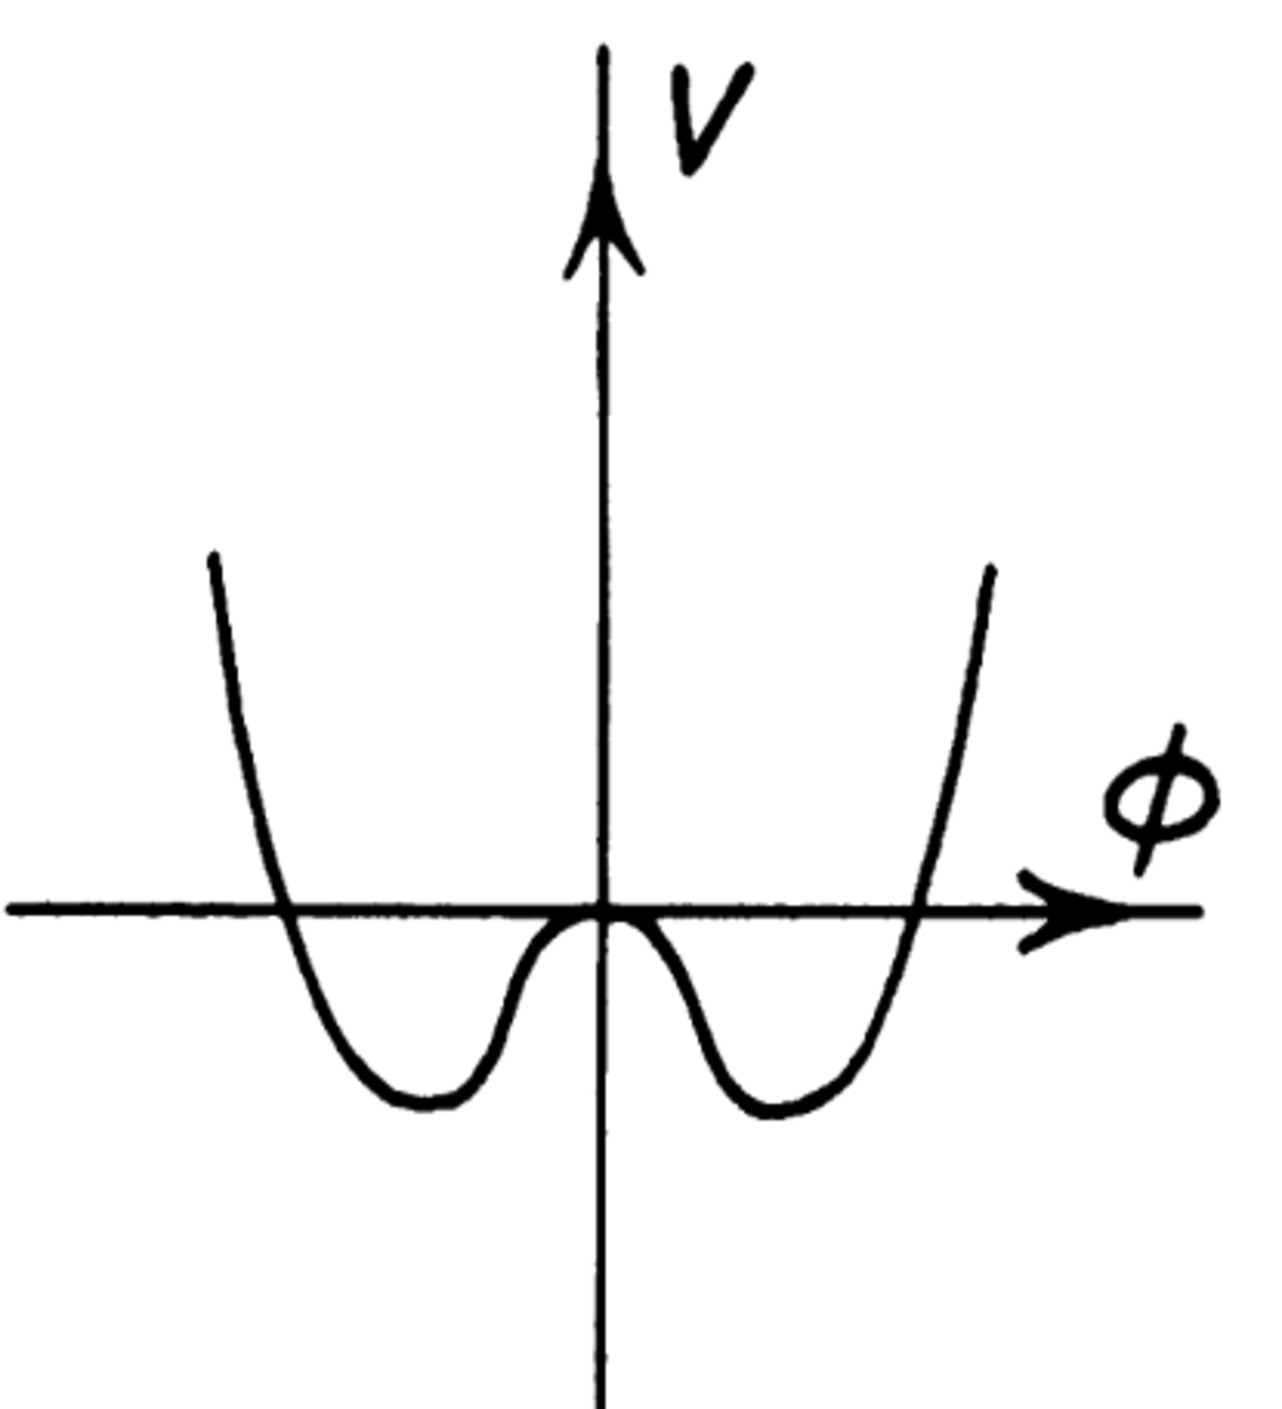
\includegraphics[height=6cm,angle=0]{IMAGEN1.pdf}
\caption{Energ'ia Potencial versus $\phi$.}
\label{fig:1}
\end{figure}
Tenemos
\begin{equation}\label{ecuacion8.4}
\phi=\pm\sqrt{\frac{-\mu^{2}}{\lambda}}\equiv v,
\end{equation}
los cuales son valores distintos de cero para $\phi$ en donde se minimiza el potencial. Luego $\phi$
  toma el valor $v$
  en el estado fundamental, $v$
  es llamado valor de expectaci'on de vac'io de $\phi$.
  El campo $\phi$
  es llamado un campo de Higgs.

Para determinar el espectro de la part'icula, debemos estudiar la teor'ia en la regi'on del m'inimo, entonces hacemos
\begin{equation}\label{ecuacion8.5}
\phi(x)=v+\eta(x),
\end{equation}
luego estamos expandiendo alrededor de $\eta=0$.
  Notemos que de igual manera pudimos haber elegido $\phi=-v+\eta(x)$,
  pero las conclusiones f'isicas son independientes de esta elecci'on, puesto que dijimos que la teor'ia es sim'etrica bajo $\phi\rightarrow-\phi$.
  Substituyendo \eqref{ecuacion8.5} en $\mathcal{L}$
  tenemos
\begin{equation}
\begin{aligned}
\mathcal{L}&=\frac{1}{2}\left(\partial^{\mu}\eta\partial_{\mu}\eta\right)-\left\{ \frac{1}{2}\mu^{2}\left[v^{2}+2\eta v+\eta^{2}\right]+\frac{1}{4}\lambda\left[v^{4}+4v^{3}\eta+6v^{2}\eta^{2}+4v\eta^{3}+\eta^{4}\right]\right\}\\ &=\frac{1}{2}\left(\partial^{\mu}\eta\partial_{\mu}\eta\right)-\left\{ \frac{v^{2}}{2}\left(\mu^{2}+\frac{1}{2}\lambda v^{2}\right)+\eta v\left(\mu^{2}+\lambda v^{2}\right)+\frac{\eta^{2}}{2}(\mu^{2}+3\lambda v^{2})+\lambda v\eta^{3}+\frac{1}{4}\lambda\eta^{4}\right\} .
\end{aligned}
\end{equation}
Usando \eqref{ecuacion8.4}, el t'ermino lineal en $\eta$
  desaparece (cerca del m'inimo), y $\mathcal{L}$
  se reduce a
\begin{equation}\label{ecuacion8.7}
\mathcal{L}=\frac{1}{2}\left(\partial^{\mu}\eta\partial_{\mu}\eta\right)-\left(\lambda v^{2}\eta^{2}+\lambda v\eta^{3}+\frac{1}{4}\lambda\eta^{4}\right)+\text{cte}.
\end{equation} 
El t'ermino con $\eta^{2}$
  tiene el signo correcto, por lo tanto puede ser interpretado como un t'ermino de masa. Este lagrangiano representa a un part'icula con masa
\begin{equation}
m_{\eta}^{2}=2\lambda v^{2}=-2\mu^{2},
\end{equation}
y con dos interacciones, una c'ubica de fuerza $\lambda v$
  y una a la cuarta de fuerza $\lambda/4$.
  Notemos que ambas dependen de $\lambda$,
  el cual es un par'ametro libre hasta donde sabemos. La constante puede ser despreciada dado que el nivel cero del potencial puede ser redefinido.

Las dos descripciones de la teor'ia, en t'erminos de $\phi$
  o $\eta$,
  debe ser equivalente si el problema es resuelto en forma exacta. Si queremos una descripci'on perturbativa es esencial perturbar alrededor del m'inimo para tener una descripci'on valida (convergente). La part'icula escalar descrita por la teor'ia con $\mu^{2}<0$
  es un escalar real, con una masa obtenida por sus propias interacciones con otros escalares, dado que el m'inimo del potencial no tiene un valor cero para el valor de expectaci'on $v$.
  No hay rastro de la simetr'ia de reflexi'on $\phi\rightarrow-\phi$
  en la ecuaci'on \eqref{ecuacion8.7}. Una memoria de esto es preservado en la interacci'on de t'ermino $\eta^{3}$. Puesto que la simetr'ia est'a quebrada, entonces cuando un vac'io espec'ifico fue elegido, el vac'io no tiene la simetr'ia del lagrangiano original. Cada vez que esto ocurre se llama \textbf{quiebre espont'aneo de simetr'ia}.
\subsection{Campo Escalar Complejo}
Supongamos que $\phi$
  es un escalar complejo 
\begin{equation}
\phi=(\phi_{1}+i\phi_{2})/\sqrt{2},
\end{equation}  
y  
\begin{equation}
\mathcal{L}=(\partial_{\mu}\phi)^{*}(\partial^{\mu}\phi)-\mu^{2}\phi^{*}\phi-\lambda(\phi^{*}\phi)^{2}.
\end{equation}
Este es invariante bajo una transformaci'on de gauge global,
\begin{equation}
\phi\rightarrow\phi^{\prime}=e^{i\chi}\phi,
\end{equation}
entonces la simetr'ia de $\mathcal{L}$
  es ahora una simetr'ia global $U(1)$
  en lugar de una reflexi'on como en el ejemplo de \ref{subseccion1} . Escribiendo en t'erminos de las componentes,
  \begin{equation}\label{ecuacion8.11}
  \mathcal{L}=\frac{1}{2}(\partial_{\mu}\phi_{1})^{2}+\frac{1}{2}(\partial_{\mu}\phi_{2})^{2}-\frac{1}{2}\mu^{2}(\phi_{1}^{2}+\phi_{2}^{2})-\frac{\lambda}{4}(\phi_{1}^{2}+\phi_{2}^{2})^{2}.
  \end{equation}
  \begin{figure}[H]
 \centering
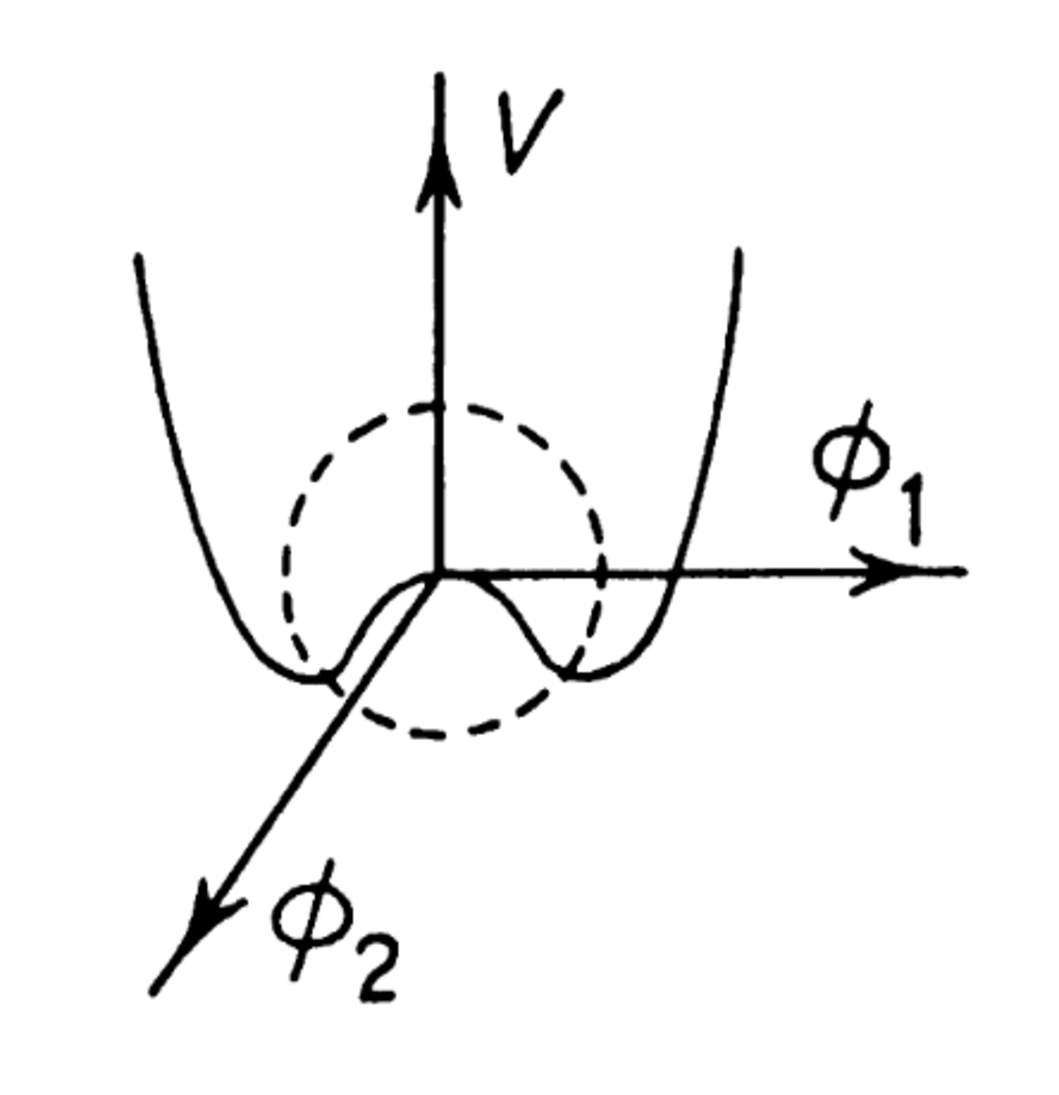
\includegraphics[height=6cm,angle=0]{IMAGEN2.pdf}
\caption{Energ'ia Potencial en funci'on de $\phi_{1}$ y $\phi_{2}$.}
\label{fig:2}
\end{figure}
 En el plano $\phi_{1},\,\phi_{2}$
  (figura \eqref{fig:2}), la energ'ia potencial es claramente un m'inimo en el origen si $\mu^{2}>0$,
  y para $\mu^{2}<0$
  el m'inimo es un circulo de radio 
\begin{equation}
\phi_{1}^{2}+\phi_{2}^{2}=\frac{-\mu^{2}}{\lambda}=v^{2}.
\end{equation}
Para analizar el caso con $\mu^{2}<0$
  tenemos que expandir cerca de $\phi_{1}^{2}+\phi_{2}^{2}=v^{2}$.
  Podemos elegir cualquier punto sobre el circulo, pero debemos elegir alg'un punto, el cual rompera la simetr'ia para la soluci'on. Escogemos, arbitrariamente, el punto $\phi_{1}=v,\,\phi_{2}=0$,
  y escribimos, con $\eta$
  y $\rho$
  reales,
  \begin{equation}
  \phi=\frac{v+\eta(x)+i\rho(x)}{\sqrt{2}}.
  \end{equation}
  Substituyendo en \eqref{ecuacion8.11}, encontramos un lagrangiano que puede ser interpretado en t'erminos de part'iculas y sus interacciones:
\begin{equation}\label{ecuacion8.14}
\mathcal{L}=\frac{1}{2}(\partial_{\mu}\rho)^{2}+\frac{1}{2}(\partial_{\mu}\eta)^{2}+\mu^{2}\eta^{2}-\lambda v\left(\eta\rho^{2}+\eta^{3}\right)-\frac{\lambda}{2}\eta^{2}\rho^{2}-\frac{\lambda}{4}\eta^{4}-\frac{\lambda}{4}\rho^{4}+\text{cte}.
\end{equation}
Los primeros t'erminos corresponden a la energ'ia cin'etica. El t'ermino $+\mu^{2}\eta^{2}$
  nos dice que el campo $\eta$
  corresponde a una part'icula de masa $m_{\eta}^{2}=2\left|\mu^{2}\right|$.
  El t'ermino en $\rho^{2}$
  a desaparecido, implicando que el campo $\rho$
  no tiene masa. Este es llamado bos'on de Goldstone. Existe un teorema general que dice, cualquiera sea una simetr'ia global continua que  est'a espontaneamente rota, el espectro contendr'a un boson de esp'in cero sin masa (bos'on de Goldstone).

T'ecnicamente es claro como el bos'on sin masa aparece. El potencial es un m'inimo a lo largo de un c'irculo. Excitaciones en la direcci'on radial requieren  tirar el potencial fuera del m'inimo y una masa est'a asociada con la curvatura del potencial. A lo largo del c'irculo el potencial es plano, entonces no hay resistencia al movimiento alrededor del c'irculo, lo cual es el resultado de la excitaci'on sin masa. La simetr'ia $U(1)$
  es rota dado la necesidad de elegir un punto en particular sobre el c'irculo sobre el cual se expande. La presencia y particular forma de los t'erminos de interacci'on en \eqref{ecuacion8.14} proveen una memoria de la simetr'ia, pero no de una forma obvia.
\section{Mecanismo de Higgs}
\subsection{Caso Abeliano}
Previamente consideramos una invariancia global de gauge. Ahora consideremos una local, hagamos el lagrangiano invariante bajo una transformaci'on local de gauge. Sabemos que la invariancia bajo una tranformacion local de gauge requiere la introducci'on de un campos $A_{\mu}$
  sin masa, y debemos escribir el lagrangiano en t'erminos de la derivada covariante. Entonces
\begin{equation}
\partial_{\mu}\rightarrow D_{\mu}=\partial_{\mu}-igA_{\mu}.
\end{equation}
El campo de gauge transforma como
\begin{equation}
A_{\mu}\rightarrow A_{\mu}^{\prime}=A_{\mu}-\frac{1}{g}\partial_{\mu}\chi(x)
\end{equation}
y $\phi$ es invariante bajo
\begin{equation}\label{ecuacion8.17}
\phi(x)\rightarrow\phi^{\prime}(x)=e^{i\chi(x)}\phi(x).
\end{equation}
As'i el lagrangiano es
\begin{equation}\label{ecuacion8.18}
\mathcal{L}=(D_{\mu}\phi)^{*}(D_{\mu}\phi)-\mu^{2}\phi^{*}\phi-\lambda(\phi^{*}\phi)^{2}-\frac{1}{4}F_{\mu\nu}F^{\mu\nu}.
\end{equation}
Para $\mu^{2}>0$
  este describe la interacci'on de una part'icula escalar cargada (con $g\equiv e$)
  de masa $\mu$
  con el campo electromagn'etico $A_{\mu}$,
  por ejemplo. Notemos que no hay un t'ermino de masa para $A_{\mu}$.
  Queremos elegir $\mu^{2}<0$
  como en las secciones anteriores. Notemos que el lagrangiano contiene cuatro campos independientes o grados de libertad, los dos campos escalares $\phi_{1}$
  y $\phi_{2}$, y los dos estados de polarizaci'on transversal del bos'on sin masa. 

La ecuaci'on \eqref{ecuacion8.17} nos dice que la teor'ia ser'a invariante bajo una transformaci'on de gauge de $\phi(x)$.
  En general $\phi$ puede ser escrito de la forma
  \begin{equation}
  \phi(x)=\eta(x)e^{-i\rho(x)}
  \end{equation}
  donde $\eta,\,\rho$
  son reales, por lo que podemos reescribir $\phi(x)$
  de la forma
  \begin{equation}
  \phi(x)=\frac{v+h(x)}{\sqrt{2}}
  \end{equation}
  con $h$
  real, habiendo usado una transformaci'on como $\phi\rightarrow e^{i\chi(x)}\phi$.
  Substituyendo en $\mathcal{L}$ tenemos
  \begin{equation}
  \begin{aligned}
  \mathcal{L}&=\frac{1}{2}[(\partial^{\mu}+igA^{\mu})(v+h)][(\partial_{\mu}-igA_{\mu})(v+h)]-\frac{\mu^{2}}{2}(v+h)^{2}-\frac{\lambda}{4}(v+h)^{4}-\frac{1}{4}F_{\mu\nu}F^{\mu\nu}\\
  &=\frac{1}{2}(\partial_{\mu}h)(\partial^{\mu}h)+\frac{1}{2}g^{2}v^{2}A_{\mu}A^{\mu}-\lambda v^{2}h^{2}-\lambda vh^{3}-\frac{\lambda}{4}h^{4}+g^{2}vhA^{\mu}A_{\mu}+\frac{1}{2}g^{2}h^{2}A_{\mu}A^{\mu}-\frac{1}{4}F_{\mu\nu}F^{\mu\nu}.
  \end{aligned}
  \end{equation}
  Aqu'i cada t'ermino puede ser interpretado. Hay un resultado interesante, ahora hay un t'ermino de masa para el bos'on de gauge!. Pero dado que comenzamos con una teor'ia invariante de gauge e hicimos solo transformaciones algebr'aicas, esperamos que la teor'ia resultante sea invariante de gauge tambi'en. La masa del bos'on de gauge es la raiz cuadrada del coeficiente de $A_{\mu}A^{\mu}/2$,
  \begin{equation}
  M_{A}=gv,
  \end{equation}
 y este es distinto de cero solo cuando la simetr'ia de gauge esta espont'aneamente quebrada por el campo de Higgs adquiriendo un valor de expectaci'on de vac'io. Entonces la teor'ia es solo invariante de gauge en un sentido restringido. El lagrangiano es invariante de gauge pero el vac'io no lo es, porque hemos escogido una direcci'on particular en $\phi_{1},\,\phi_{2}$ para el potencial m'inimo.
 El espectro es ahora un unico boson de Higgs real $h$,
  con masa $\sqrt{(2\lambda v^{2})}$, varias interacciones propias e interacciones c'ubicas y cuarticas con el campo de gauge $A_{\mu}$,
  m'as un bos'on $A_{\mu}$.
  Dado que el bos'on masivo tiene 3 estados de spin ( correspondientes a $J_{z}=1,\,0,\,-1$)
  el n'umero de campos independientes es a'un cuatro, lo que es consistente.

Lo que ha ocurrido aqu'i es que el bos'on de Goldstone de la secci'on anterior se ha convertido en el estado de polarizaci'on longitudinal del bos'on de gauge. 'Este fen'omeno se le refiere a veces diciendo que el bos'on de gauge se \textit{come} al bos'on de Goldstone. El mecanismo anterior es llamado como \textbf{Mecanismo de Higgs}.
\begin{thebibliography}{99}

\addcontentsline{toc}{chapter}{Bibliograf'ia}

\bibitem{MTW}  C.W. Misner, K.S. Thorne and J.A. Wheleer, \emph{Gravitation}, W.H. Freeman and Company (1973).

\bibitem{Gilmore}  R. Gilmore, \emph{Lie Groups, Lie Algebras, and some of
Their Applications}, John Wiley \& Sons, Inc. (1974).

\bibitem{BS}  S. Browne and D. \v {S}ija\v {c}ki, ``On the Irreducible
Representations of the Lorentz Group'', \emph{Ann. Phys.} (N.Y.) \textbf{99}
92--126 (1976).

\bibitem{Cornwell}  J.F Cornwell, \emph{Group Theory in Physics, Vol II},
Academic Press Ltd. (1984).

\bibitem{Ham}  M. Hamermesh, \emph{Group Theory and its application to
physical problems}, Addison-Wesley Publishing Company, Inc. (1962).

\bibitem{Das} Ashok Das, \emph{Lectures on Quantum Field Theory}, Univerity of Rochester, USA, 2008.
\bibitem{kaku} Michio Kaku, \emph{Quantum Field Theory: A Modern Introduction}, Oxford University Press, 1993.
\bibitem{G.Rubilar} Guillermo F. Rubilar, \emph{Apuntes Curso Electrodin'amica}, Universidad de Concepci'on. \url{https://sites.google.com/site/apuntesdecienciasfisicas/}.
\bibitem{jackson} J.D. Jackson, \emph{Classical Electrodynamics}, John Wiley \& Sons, Inc., 1962.
\bibitem{PS} Patricio Salgado, \emph{Apuntes Quiebre Espont'aneo de Simetr'ia}, Universidad de Concepci'on.

\bibitem{GK} Gordon Kane, \emph{Modern Elementary Particle Physics}, Addison-Wesley Publishing Company, Inc. (1993).

\end{thebibliography}

\end{document}
